\documentclass[a4paper,11pt]{article}
\usepackage[a4paper,left=0.99in, right=0.99in,top=1.2in, bottom=1.2in]{geometry}

\usepackage{common-defs}
\usepackage{hyperref}
\usepackage{cite}
\usepackage{graphicx}
\usepackage{bm,braket}
\usepackage{amsmath}
\numberwithin{equation}{section}

\newcommand{\question}[1]{{\bf Question:} #1}
\newcommand{\slashnbar}{\slashed{\bar n}}
\newcommand{\mixed}{{M}}
\newcommand{\mycite}[1]{{\footnote{\tt  #1}}}
\newcommand{\Litwo}{{\text{Li}_2}}
\newcommand{\Lithree}{{\text{Li}_3}}
\newcommand{\bfS}{\bm{S}}
\newcommand{\bfH}{\bm{H}}
\newcommand{\bfw}{\bm{w}}
\newcommand{\bfZ}{\bm{Z}}

\newcommand{\bJ}{\mathbf{J}}
\newcommand{\bT}{\mathbf{T}}


\newcommand{\Rp}{\right)}
\newcommand{\Lp}{\left(}
\newcommand{\Rb}{\right]}
\newcommand{\Lb}{\left[}



\newcommand{\bfgamma}{\bm{\gamma}}
\newcommand{\bfGamma}{\bm{\Gamma}}
\newcommand{\bfI}{\bm{1}}
\newcommand{\idop}{{1\hspace{-4pt} 1}}
\newcommand{\wii}[1]{{\bfw_{i\bar i}^{#1}}}
\newcommand{\kp}{k_+}
\newcommand{\lp}{l_+}
\newcommand{\dd}{\text{d}}
\newcommand{\smallcomment}[1]{{\small \it (#1)}}
\newcommand{\ldot}{\!\cdot\!}
\newcommand{\bn}{\overline{n}}
\newcommand{\pola}{\varepsilon}
\newcommand{\bd}[1]{\mathbf{#1}}


\newcommand{\eps}{\epsilon}
\newcommand{\veps}{\varepsilon}

\newcommand{\CC}[1]{\mathbf{T}_{#1}}



\allowdisplaybreaks

\title{Integration of soft function at NNLO}
\author{Rene Angeles-Martinez}
%-----------------------------------------------------------------------------
\begin{document}
\maketitle

\noindent \rule{\textwidth}{1pt}
\tableofcontents
\noindent \rule{\textwidth}{1pt}

\newpage

%-----------------------------------------------------------------------------
\section{Introduction}

Integration of the soft function relevant to small $q_t$ resummation is addressed. 
%

%-----------------------------------------------------------------------------
\newpage



\section{NLO graph contribution to S1bare in momentum space}

\begin{equation}
S_{d}= \frac{2\pi^{(d+1)/2}}{\Gamma[(d+1)/2]}
\end{equation}

\begin{align}
& q_T^{-2-2\alpha}
\underbrace{\left( 
\frac{(2\pi)^{d-2}}{(2\pi)^{d/2-1}}\right)}_{\text{Fourier prefactors}}
\underbrace{\left( (4\pi)^2 
\frac{e^{\eps \gamma_E}}{(4\pi)^\eps} \right)}_{\text{MSbar}}
\underbrace{ \left( \frac{2}{S_{1-2\eps}} \right)}_{\text{qT azimuthal average}}
\mathbf{I}_{ij}
\end{align}

\begin{align*}
\mathbf{I}_{ij}=\frac{T_i\cdot T_j}{d_R}\equiv\int 
\frac{d^d k}{(2\pi)^{d-1}k_+^\alpha}\delta(k^2)\theta(k^0)
\frac{-p_i\cdot p_j}{p_i\cdot k\, p_j\cdot k}
\delta(k_T^2-1)
\end{align*}




\section{Double cuts over the boundary}

In this section, we consider the most general integral that appear when dealing with 
diagrams with double cuts. These are all of the form
%
\begin{equation}
  \int \frac{ \frac{\dd^d k}{(2\pi)^{d-1}}\, \frac{\dd^d l}{(2\pi)^{d-1}} \,  \Big( \delta^+(k^2) \delta^+(l^2) \Big) \,
            \Big(\delta(|k_\perp+l_\perp|^2-1)\Big)}{(\text{Rapidty})} \times \text{Graph part}\,,
  \label{eq:master}
\end{equation}
where $\delta^{+}(k)\equiv \theta(k^0)\delta(k^2)$.
%
%-----------------------------------------------------------------------------
\subsection{Integration of on-shell and observable condition}

It is convenient to introduce the following vectors
%
\begin{equation}
  n = (1,0,0,1)\,,\quad \nbar = (1,0,0,-1)\,, \qquad n\cdot \nbar = 2\,,
  \qquad n^2 = \nbar^2 = 0\,,
  \label{eq:nnbar-defs}
\end{equation}
%
which are the directions of the colliding partons, and
%
\begin{eqnarray}
  k^\mu 
  & =  &
  n\cdot k \frac{\nbar^\mu}{2} + \nbar \cdot k \frac{n^\mu}{2} + 
  k_\perp^\mu \\
  & \equiv & 
  k^+ \frac{\nbar^\mu}{2} +  k^- \frac{n^\mu}{2} + k_\perp^\mu\,.
\end{eqnarray}
Then
\begin{align}
&k^+=k^0-k^z\qquad k^-=k^0+k^z \\
&k\cdot l= \frac{k^+ l^-}{2}+\frac{k^- l^+}{2}- l_T\cdot k_T.
\end{align}
Sebastian convention for the initial state partons is $p_1=p_1^0 n$ and $p_2=p_2^0 \bar{n}$. 
The integration measures in the transverse plane reads 
\footnote{This angle arises from  
$\int \dd^{d-2} k_T=\int_0^\infty \dd k_T k_T^{d-3} \int_{S_{d-3}}\dd \Omega  $ with
$\int_{S_{d-3}} \dd \Omega= S_{d-4}\int_{-1}^{1}\dd \cos\phi \sin^{-1-2 \eps}$, where $S_{2\eps}= \frac{2(4\pi)^{-\eps} \Gamma[1-\eps]}{\Gamma[1-2\eps]}$. Sometimes, to integrate this angle it is convenient
to change $\cos\phi \to 1-2\eta$, i.e. 
$\int_{-1}^{1}\dd \cos\phi \sin^{-1-2 \eps}
=\int_{0}^{1}\dd \eta\, 2(4\eta(1-\eta))^{-1/2- \eps} $.}
%
\begin{eqnarray}
  d^{d-2} k_\perp & = & 
  \Omega_{1-2\epsilon}\,
  k_T^{1-2\epsilon} \sin^{-2\epsilon}\! \phi\, d k_T\, d\phi\,,
  \\
  d^{d-2} l_\perp & = & 
  \Omega_{2-2\epsilon}\,
  l_T^{1-2\epsilon} d l_T\,.
  %\label{eq:}
\end{eqnarray}
where $\phi$ the latter is the angle between transverse components of gluons four-momenta. 
%
To integrate the observable delta function one can observe that
%
\begin{align}
 \delta\left(|k_\perp+l_\perp|^2-1\right)=
\frac{\theta(k_\perp+l_\perp-1) \theta(1-|k_\perp-l_\perp|)}
{2k_\perp l_\perp} \delta\left(\cos\phi -\frac{1- k_\perp^2-l_\perp^2}{2k_\perp l_\perp }\right).
\end{align}
%
Using this delta function to integrate $\phi$ and the on-shell conditions to integrate over $l^-$ and $l^+$, 
Eq.~\eqref{eq:master} can be written as
%
\begin{align}
\frac{\Omega_{1-2\epsilon}}{(2\pi)^{d-1}} \frac{\Omega_{2-2\epsilon} }{(2\pi)^{d-1}}
\int  &k_\perp^{1-2\epsilon} d l_\perp l_\perp^{1-2\epsilon} d l_\perp
	    \Big( \frac{dk_+}{k_+^{1+\alpha}} \frac{dl_+}{l_+^{1+\alpha}} \Big) \,
            \left\{
            \frac{1}{2k_\perp\, l_\perp}
            \left( 
            \frac{(1-(k_\perp+l_\perp)^2)(1-(k_\perp-l_\perp)^2)}{4k_\perp^2l_\perp^2}
            \right)^{-1/2-\epsilon}
            \right\}\nonumber\\
           &\times   \text{Graph part} \,,
  \label{eq:master2}
\end{align}
%
where the domain of integration is understood to satisfy the theta and delta function constrains. From now on, we shall only focus on these regions. Also remember that $\Omega_{d-1}\equiv 2\pi^{d/2}/\Gamma[d/2]$



\subsection{Relevant regions}

In this section, we present the regions of the integration domain in which the integrand of Eq.~\eqref{eq:master2} vanishes.

\subsubsection{Propagators of incoming partons}
%In general, rapidity regulators and eikonal propagators related to incoming 
%partons only vanishes when the light cone coordinates of soft gluons 
%vanishes, and this occurs in three different regions described below.
\begin{itemize}
\item Soft region: $\lambda\, ( k^+, k_\perp^2/(2k^+),  k_\perp ),\, \lambda\ll1$. Within the integration domain, this constrain implies $l_\perp\to 1$, i.e. gluon $l$ cannot be soft or collinear with the incoming partons.
\item Collinear region: $(  k^+, \lambda^2 k_\perp^2/(2k^+), \lambda k_\perp )$. Within the integration domain, this constrain implies $l_\perp\to 1$, i.e. gluon $l$ cannot be soft or collinear with the incoming partons. Note that a second global re-scaling would make gluon $k$ soft, i.e. the soft and collinear regions are not disjoint. 
\item "Rapidity region": $(\lambda  k^+, k_\perp^2/ (\lambda 2k^+),  k_\perp )$. Note that parton $k$ is not necessarily soft\footnote{A second global re-scaling would make it soft.}. Also note that gluon $k$ can not be collinear, as a collinear re-scaling would invalidate the first scaling.
%Meanwhile, gluon $l$ can be soft and be wide angle or collinear with an incoming parton. 
\end{itemize}
The rapidity region leads to divergences in the Eikonal approximation but 
not for the exact theory. 

\subsubsection{Eikonal propagators of $(t,\bar{t})$}

Clearly, these only vanish in the soft region, e.g. $(\lambda\, k^+,\lambda\, k_\perp^2/(2k^+)$ and $l_\perp\to 1$, and it is convenient to write these propagators as
\begin{align}
k\cdot v_i= k^0   \frac{k \cdot v_i}{k_0} = \sqrt{2}\left(k^++\frac{k_\perp^2}{2k^+}\right)   \frac{k \cdot v_i}{k_0}.
\end{align} 

\subsubsection{Divergences of exact propagators}

After evaluation of the azimuth $\phi$, this exact propagator reads
%
\begin{align}
2k\cdot l=   \left(-1 + (k_\perp^2 (k^+ + l^+))/k^+ + ((k^+ + l^+) l_\perp^2)/l^+\right)
\end{align}
%
One can show that\footnote{See mathematica notebook} the only points, in the domain of integration, for which 
this propagators identically vanish are
\begin{align}
\left\{�k_\perp=\frac{k^+}{k^+ + l^+}, l_\perp=\frac{l^+}{k^+ + l^+} \right\}.
\end{align}
Note that only one of the two gluons can have vanishing transverse momentum.





%%The boundary integral can be parametrized with $k_+$, $k_-$, $l_+$, $l_-$,
%%$k_T$, $l_T$ and $\phi$, where the latter is the angle between transverse
%%components of gluons four-momenta. The integration measures in the transverse
%%plane read
%%%
%%\begin{eqnarray}
%%  d^{d-2} k_\perp & = & 
%%  \Omega_{1-2\epsilon}\,
%%  k_T^{1-2\epsilon} \sin^{-2\epsilon}\! \phi\, d k_T\, d\phi\,,
%%  \\
%%  d^{d-2} l_\perp & = & 
%%  \Omega_{2-2\epsilon}\,
%%  l_T^{1-2\epsilon} d l_T\,.
%%  %\label{eq:}
%%\end{eqnarray}
%%%
%%\smallcomment{Possible issue with factor 1/2 related to $[0,2\pi]$ range of
%%$\phi$.}\\
%%%
%%It is convenient to replace the angular variable $\phi$ by
%%%
%%\begin{equation}
%%  \eta = \frac{1-\cos\phi}{2}\,.
%%  %\label{eq:}
%%\end{equation}
%%%
%%Then, the whole measure takes the form
%%%
%%\begin{equation}
%%  \dd^d k\, \dd^d l =
%%  4^{-\epsilon}
%%  \Omega_{1-2\epsilon}\,
%%  \Omega_{2-2\epsilon}\;
%%  k_T^{1-2\epsilon} \,
%%  l_T^{1-2\epsilon} 
%%  \big((1-\eta)\eta \big)^{-\frac12-\epsilon}
%%  dk_+ dk_- dl_+ dl_-
%%  d k_T\, 
%%  d l_T\,
%%  d\eta\,.
%%  %\label{eq:}
%%\end{equation}
%%%
%%After performing integrations over $k_-$, $l_-$ and $\eta$, we are left with
%%the following form of the boundary integral
%%%
%%\begin{equation}
%%  I =
%%  \Sigma
%%  \int dk_+ dl_+ dk_T dl_T
%%  \frac{k_+^{-1-\alpha}\, l_+^{1-\alpha} k_T l_T \,
%%  \Big\{\big[1-(k_T-l_T)^2\big]\big[1-(k_T+l_T)^2\big]
%%  \Big\}^{-\frac12-\epsilon}
%%  }{(l_+^2+l_T^2)
%%  \big(k_T^2 k_+ l_+ +l_T^2 k_+ l_+ + k_T^2 l_+^2 + l_T^2 k_+^2 - k_+ l_+
%%  \big)
%%  }\,,
%%  %\label{eq:}
%%\end{equation}
%%%
%%where $\Sigma$ contains all the constants and the $\delta$ functions generated
%%the following relations
%%%
%%\begin{equation}
%%  k_- = \frac{k_T^2}{k_+}\,, \qquad \qquad
%%  l_- = \frac{l_T^2}{l_+},
%%  %\label{eq:}
%%\end{equation}
%%%
%%and
%%\begin{equation}
%%  | k_T - l_T | \leq 1\,,
%%  \qquad \land \qquad
%%   k_T + l_T  \geq 1\,.
%%  \label{eq:kTlT-region}
%%\end{equation}
%%%
%%The last pair of relations defines the integration region in the $(k_T, l_T)$
%%plane.  This region is depicted in Fig.~\ref{fig:trans-regions}~(left).  The
%%first inequality in (\ref{eq:kTlT-region}) corresponds to the two solid (red)
%%lines, while the second inequality corresponds to the dotted (blue) line.
%%
%%\begin{figure}[t]
%%  \begin{center}
%%    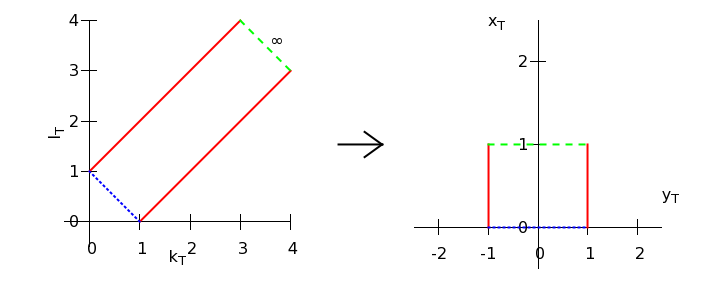
\includegraphics[width=0.99\textwidth]{plots/transverse-phase-space.png}
%%  \end{center}
%%  \caption{
%%  Change of integration region after transformation of transverse coordinates.
%%  }
%%  \label{fig:trans-regions}
%%\end{figure}
%%
%%The integral $I$ is divergent in the following cases:
%%%
%%\begin{enumerate}
%%  \item
%%    $k_+ \to 0$, 
%%    rapidity divergence for gluon $g(k)$
%%  \item 
%%    $k_+ \to 0,\ l_+ \to 0$, ???
%%  \item
%%    $l_+ \to 0,\ l_T \to 0$, 
%%    soft divergence for gluon $g(l)$
%%  \item
%%    $k_T \to \displaystyle \frac{k_+ }{k_+ + l_+},
%%    \ l_T \to \frac{l_+ }{k_+ + l_+}$,
%%    collinear divergence of 3-gluon vertex
%%\end{enumerate}
%%%
%%Let us call the cases 3. and 4. the ``mixed divergences''.
%%
%%We would like to transform the integration region in the $(\kp, \lp, k_T, l_T)$
%%space into a hypercube and, if necessary, split it such that each of resulting
%%integrals $\int \prod_i d x_i f(\{x_i\})$ has singularities only in the limits
%%$x_i \to 0$.
%%%
%%We achieve the above in the following steps:
%% 
%%%------------------------------------
%%\subsubsection*{Step 1}
%%
%%The transverse variables $(k_T, l_T)$ are transformed to new variables 
%%$(x_T, y_T)$ with the following replacements
%%%
%%\begin{equation}
%%  k_T = \frac{1+y_T-x_T y_T}{2(1-x_T)}\,,
%%  \qquad \qquad
%%  l_T = \frac{1-y_T+x_T y_T}{2(1-x_T)}\,,
%%  %\label{eq:}
%%\end{equation}
%%%
%%and the inverse transformation reads
%%\begin{equation}
%%  x_T = 1-\frac{1}{k_T+l_T}\,,
%%  \qquad \qquad
%%  y_T = k_T-l_T\,.
%%  %\label{eq:}
%%\end{equation}
%%
%%This results in change of the integration region from the one shown in
%%Fig.~\ref{fig:trans-regions}~(left) to that of
%%Fig.~\ref{fig:trans-regions}~(right). The latter corresponds to
%%%
%%\begin{equation}
%%  0 \leq x_T \leq 1
%%  \qquad \land \qquad
%%  -1 \leq y_T \leq 1\,.
%%  %\label{eq:}
%%\end{equation}
%%
%%The mixed divergences  now happen at
%%%
%%\begin{enumerate}
%%  \setcounter{enumi}{2}
%%  \item
%%    $l_+ \to 0,\ x_T \to 0,\ y_T \to 1$,
%%  \item
%%    $x_T \to 0,\ y_T \to \displaystyle \frac{\kp-\lp}{\kp+\lp}$\,.
%%\end{enumerate}
%%%
%%The last divergence occurs on a manifold inside the integration region. This
%%manifold is depicted in Fig.~\ref{fig:yTmanifold}.
%%
%%\begin{figure}[t]
%%  \begin{center}
%%    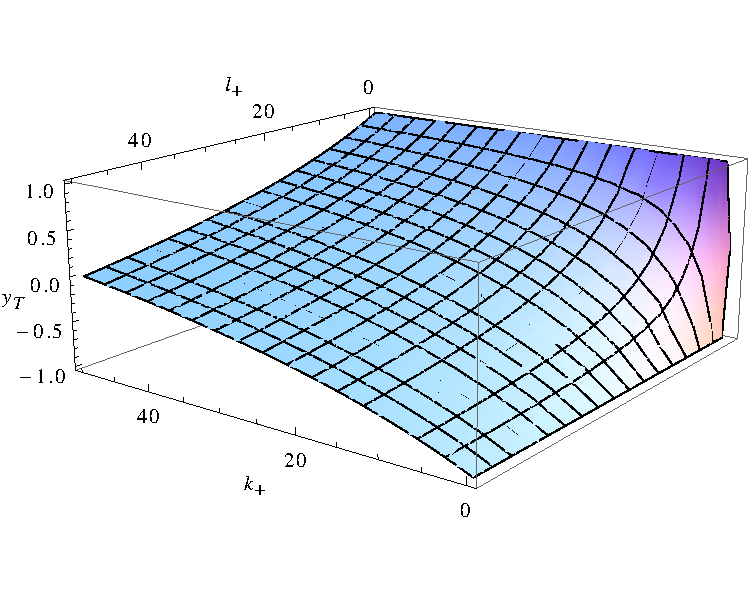
\includegraphics[width=0.49\textwidth]{plots/yTmanifold.pdf}
%%  \end{center}
%%  \caption{
%%  Manifold where the boundary integral becomes singular.
%%  }
%%  \label{fig:yTmanifold}
%%\end{figure}
%%
%%%------------------------------------
%%\subsubsection*{Step 2}
%%
%%In order to transform the manifold singularity into endpoint singularity, we
%%split the integration region in variable $y_T$ precisely on the manifold of
%%Fig.~\ref{fig:yTmanifold}
%%%
%%\begin{eqnarray}
%%  I & =  & 
%%  \int_0^\infty\!\!\! d\kp
%%  \int_0^\infty\!\!\! d\lp
%%  \int_0^1\!\!\! d x_T
%%  \int_{-1}^1\!\!\! d y_T\
%%  \tilde I(\kp, \lp, x_T, y_T)
%%  \nonumber \\
%%  & = &
%%  \int  d\kp d\lp d x_T
%%  \int_{-1}^{c(\kp, \lp)}\!\!\! d y_T\
%%  \tilde I(\kp, \lp, x_T, y_T)
%%  +
%%  \int  d\kp d\lp d x_T
%%  \int_{c(\kp, \lp)}^{1}\!\!\! d y_T\
%%  \tilde I(\kp, \lp, x_T, y_T)
%%  \nonumber \\
%%  & \equiv &
%%  I_d + I_u\,,
%%  %\label{eq:}
%%\end{eqnarray}
%%%
%%where
%%%
%%\begin{equation}
%%  c(\kp, \lp) = \frac{\kp-\lp}{\kp+\lp}\,.
%%  %\label{eq:}
%%\end{equation}
%%
%%Now, we use two different parametrizations
%%%
%%\begin{equation}
%%  y_T = \frac{\kp-\lp + 2 \lp \bar y_T}{\kp+\lp}\,,
%%  \qquad \qquad
%%  \bar y_T = \frac{y_T-c(\kp,\lp)}{1-c(\kp,\lp)},
%%  \qquad 
%%  \text{for}\quad I_u\,,
%%  %\label{eq:}
%%\end{equation}
%%%
%%and
%%%
%%\begin{equation}
%%  y_T = \frac{\kp-\lp - 2 \lp \bar y_T}{\kp+\lp}\,,
%%  \qquad
%%  \bar y_T = \frac{y_T-c(\kp,\lp)}{-1-c(\kp,\lp)},
%%  \qquad \qquad
%%  \text{for}\quad I_d\,.
%%  %\label{eq:}
%%\end{equation}
%%%
%%Hence, we obtain
%%%
%%\begin{eqnarray}
%% I_d  & =  &
%%  \int_0^\infty\!\!\! d\kp
%%  \int_0^\infty\!\!\! d\lp
%%  \int_0^1\!\!\! d x_T
%%  \int_{0}^1\!\!\! d \bar y_T\
%%  \tilde I_1(\kp, \lp, x_T, \bar y_T)\,,
%%  \\
%% I_u  & =  &
%%  \int_0^\infty\!\!\! d\kp
%%  \int_0^\infty\!\!\! d\lp
%%  \int_0^1\!\!\! d x_T
%%  \int_{0}^1\!\!\! d \bar y_T\
%%  \tilde I_2(\kp, \lp, x_T, \bar y_T)\,.
%%  %\label{eq:}
%%\end{eqnarray}
%%
%%With the above changes, the mixed singularities happen at
%%%
%%\begin{enumerate}
%%  \setcounter{enumi}{2}
%%  \item
%%    $l_+ \to 0,\ x_T \to 0,\ \bar y_T \to 1$,
%%  \item
%%    $x_T \to 0,\ \bar y_T \to 0$
%%\end{enumerate}
%%%
%%for $I_u$ and
%%%
%%\begin{enumerate}
%%  \setcounter{enumi}{2}
%%  \item
%%    $x_T \to 0,\ \bar y_T \to 0$
%%\end{enumerate}
%%%
%%for $I_d$ and.
%%%
%%We see that, in the case of $I_u$, the integral can be divergent at both ends of
%%$\bar y_T$.
%%
%%%------------------------------------
%%\subsubsection*{Step 3}
%%
%%In order to move all singularities to the limit $x_i \to 0$, we split $I_u$ at 
%%$\bar y_T = \frac12$
%%%
%%\begin{equation}
%% I_u = \int_0^1 d \bar y_T\, \tilde I =
%% \int_0^\frac12 d \bar y_T\, \tilde I +
%% \int_\frac12^1 d \bar y_T\, \tilde I \equiv I_{u0} + I_{u1}\,.
%%  %\label{eq:}
%%\end{equation}
%%%
%%Then, we apply the following transformations
%%%
%%\begin{equation}
%%  \tilde y_T = 2(1-\bar y_T)\,,
%%  \qquad \qquad
%%  \bar y_T = 1-\frac{\tilde y_T}{2}\,,
%%  \qquad 
%%  \text{for}\quad I_{u1}\,,
%%  %\label{eq:}
%%\end{equation}
%%%
%%and
%%%
%%\begin{equation}
%%  \tilde y_T = 2 \bar y_T\,,
%%  \qquad \qquad
%%  \bar y_T = \frac{\tilde y_T}{2}\,,
%%  \qquad 
%%  \text{for}\quad I_{u0}\,.
%%  %\label{eq:}
%%\end{equation}
%%%
%%At this point, we have the following mixed singularities:
%%
%%\begin{displaymath}
%%  \begin{array}{ll}
%%   \text{for }  I_{u1}: &
%%   l_+ \to 0,\ x_T \to 0,\ y_T \to 0,
%%   \\
%%    \text{for } I_{u0} \text{ and } I_d: &
%%    x_T \to 0,\  y_T \to 0\,,
%%    \\[0.5em]
%%  \end{array}
%%\end{displaymath}
%% 
%%\noindent
%%where we dropped tildes and bars for simplicity of notation.
%%
%%%------------------------------------
%%\subsubsection*{Step 4}
%%
%%In the last step, we compress the ranges of the $\kp$ and $\lp$ integrals by the
%%transformation
%%%
%%\begin{equation}
%%  \kp = \frac{x}{1-x}\,, 
%%  \qquad \qquad
%%  \lp = \frac{y}{1-y}\,, 
%%\end{equation}
%%%
%%whose inverse reads
%%\begin{equation}
%%  x = \frac{\kp}{1+\kp}\,, 
%%  \qquad \qquad
%%  y = \frac{\lp}{1+\lp}\,.
%%\end{equation}
%%
%%Hence, finally, our boundary integral is a sum of three contributions
%%%
%%\begin{equation}
%%  I = I_d + I_{u0} + I_{u1}\,,
%%  %\label{eq:}
%%\end{equation}
%%%
%%which are singular in the following limits: \vspace{10pt}
%%
%%\noindent
%%$I_d$:
%%%
%%\begin{enumerate}
%%  \item
%%  $x \to 0$\,,
%%  \vspace{-5pt}
%%  \item
%%  $x \to 0,\ y \to 0$\,,
%%  \vspace{-5pt}
%%  \item
%%   $ x_T \to 0,\  y_T \to 0$\,,
%%\end{enumerate}
%%
%%\noindent
%%$I_{u0}$:
%%%
%%\begin{enumerate}
%%  \item
%%  $x \to 0$\,,
%%  \vspace{-5pt}
%%  \item
%%  $x \to 0,\ y \to 0$\,,
%%  \vspace{-5pt}
%%  \item
%%   $ x_T \to 0,\  y_T \to 0$\,,
%%\end{enumerate}
%%
%%\noindent
%%$I_{u1}$:
%%%
%%\begin{enumerate}
%%  \item
%%  $x \to 0$\,,
%%  \vspace{-5pt}
%%  \item
%%  $x \to 0,\ y \to 0$\,,
%%  \vspace{-5pt}
%%  \item
%%   $y \to 0,\ x_T \to 0,\ y_T \to 0$\,.
%%\end{enumerate}


%-----------------------------------------------------------------------------

%-----------------------------------------------------------------------------
\newpage
\section{Analytical integration on the boundary }

In this section, we are slopy with ep prefactor. 

We perform analytical integration of the following integral over the 
boundary $\beta=1$\footnote{i.e., $\{v_3,v_4\}$ only have energy components.}: 
\begin{equation}
I_1=  \int  \dd^d k\, \dd^d l\,  	
	\Big( \delta^+(k^2) \delta^+(l^2) \Big) \,            
         \Big(\delta(|k_\perp+l_\perp|^2-1)\Big) 
         \times\left[ \frac1{
            (n \cdot l\, n\cdot k)^{\alpha}\,
            n\ldot l\, \bn\ldot k\,
            v_3\ldot l\, v_4\ldot k} \right]. 
\end{equation}

%\begin{equation}
%I_2=  \int \frac{\dd^d k\, \dd^d l\,  
%  	\left(\frac{\nu_k}{n \cdot k} \right)^{\alpha}
%	\left(\frac{\nu_l}{n \cdot l} \right)^{\alpha}
%	\Big( \delta^+(k^2) \delta^+(l^2) \Big) \,
%            \Big(\delta(|k_\perp+l_\perp|^2-1)\Big)}{
%            (n \cdot k\, n\cdot l)^{\alpha}\,
%            \bn\ldot(k+l)\, \bn\ldot k\,
%            p_3\ldot(k+l)\, p_3\ldot k }\,
%\end{equation}

Integrating out the delta function one gets 
\begin{align}
I_1 (v_3^0 v_4^0) = \Omega_{1-2\epsilon} \Omega_{2-2\epsilon} 
\int&  k_\perp^{1-2\epsilon} \dd k_\perp l_\perp^{1-2\epsilon} 
	    d l_\perp \frac{\dd k^+}{k^+} \frac{\dd l^+}{l^+}	     
	    \left\{
            \frac{1}{2k_\perp\, l_\perp}
            \left( 
            \frac{(1-(k_\perp+l_\perp)^2)(1-(k_\perp-l_\perp)^2)}{4k_\perp^2l_\perp^2}
            \right)^{-1/2-\epsilon}
            \right\} 
            \nonumber\\
            &\times \theta(k_\perp+l_\perp-1) \theta(1-|k_\perp-l_\perp|)
            \nonumber\\            
            &\times 4 \left[ \frac{ k_+^2l_+ }{ (k^+ l^+)^\alpha\, \, l^+\,  k_\perp^2
            \, (k_+^2 +k_\perp^2) \, (l_+^2 +l_\perp^2)   }\right]
 \end{align}
 The first two lines lines are common to all scalar integrals, they correspond to measure and observable factors.   
 After trivial re-arrangements this integral can be re-expressed as
\begin{align}            
            = 2^{1+2\epsilon} \Omega_{1-2\epsilon} \Omega_{2-2\epsilon} 
	    \int&  \dd k_\perp  \dd l_\perp \dd l^+ \dd k^+
	     \frac{\left( f(k_\perp, l_\perp)\right)^{-1/2-\epsilon}}
	    {(k^+ l^+)^\alpha}  \theta(k_\perp+l_\perp-1) \theta(|k_\perp-l_\perp|-1)
	    \nonumber\\
	    &\times 4 \left(\frac{k^+ }{k_\perp(k_+^2 +k_\perp^2) } \right)     
	    \left( \frac{l_\perp}{  l^+(l_+^2 +l_\perp^2)}\right) \,.
\end{align}
where $f(k_\perp, l_\perp)=  (1-(k_\perp+l_\perp)^2)(1-(k_\perp-l_\perp)^2)$. From this expression we can see that the integral contains divergences in the following regions 
\begin{itemize}
\item  $k_\perp\to \infty $. This ``rapidity'' divergence is regularised only if $\alpha>0$
\item  $k_\perp,k^+\to 0 $ and $k_\perp\to 0$.
\item  $l_\perp,l^+\to 0$ and $l_+\to0$. This latter
``rapidity'' divergence is regularised only if $\alpha<0$
\end{itemize}
Hence, this integral is not a simple function of $\alpha$. The integration over $l^+$ is straightforward by assuming $\alpha>0$, and performing the remaining integration assuming that $\alpha,\epsilon$ are small and such that $\alpha<2\epsilon$. The analytic expression 
\begin{align}
\frac {I_1}{ (p_3^0 p_4^0)  \Omega_{1-2\epsilon} \Omega_{2-2\epsilon} }=
\frac{\pi ^3 \csc ^2\left(\frac{\pi  \alpha }{2}\right) 2^{\alpha +2 \epsilon-1} \Gamma \left(\frac{1}{2}-\epsilon\right) \Gamma \left(-\epsilon-\frac{\alpha }{2}\right) \Gamma (\epsilon+\alpha +1)}{\Gamma \left(\frac{\alpha }{2}+1\right)^2 \Gamma \left(-\epsilon-\frac{\alpha }{2}+\frac{1}{2}\right)} 
\label{eq:analytic}
\end{align}
On the other hand, this same integral can be computed by means of sector decomposion. The following mappings 
are needed to get rid of overlapping singularities
\begin{enumerate}
\item 
\begin{align}
  k_T &= \frac{1+y_T-x_T y_T}{2(1-x_T)}\,,
  \qquad \qquad
  l_T = \frac{1-y_T+x_T y_T}{2(1-x_T)}\,, \\
  x_T &= 1-\frac{1}{k_T+l_T}\,,
  \qquad \qquad
  y_T = k_T-l_T\,.
\end{align}
Where the new variables should be integrated over the domain $0\le x_T\in \le 1, |y_T|\le 1$. 
The points $k_T\to 0$ and $l_T\to 0$ in the new variables have moved to $x_T\to 0$ with 
$y_T=-1$ and $y_T=1$. 
\item In the present case, there is not manifold singularity but an analogous mapping is needed to separate the singularities at   $y_T=-1$ and $y_T=1$. For this propose, we simple break the integration domain into 
$y_T\in [0,1]$ and $y_T= [-1,0]$ and make the transformation $y_T \to -y_T$ for the latter case. 
\item The third mapping separates regions with finite and vanishing transverse momentum, rendering four integrals
For this propose, we break the integration domain at $y_T=1/2$ and apply the transformations
%
\begin{equation}
  \tilde y_T = 2(1- y_T)\,,
\end{equation}
%
and
%
\begin{equation}
  \tilde y_T = 2  y_T\,,
\end{equation}
%
This completes the set of transformations required for the transverse components. 
\item Now one needs to compress the domain of integration of the plus components, this is achieved by 
the transformations
%
\begin{equation}
  \kp = \frac{x}{1-x}\,, 
  \qquad \qquad
  \lp = \frac{y}{1-y}\,, 
\end{equation}
%
whose inverse reads
\begin{equation}
  x = \frac{\kp}{1+\kp}\,, 
  \qquad \qquad
  y = \frac{\lp}{1+\lp}\,.
\end{equation}
The domain of integration of the new variables is $x,y\in [0,1] $. 
\item Note that $x=0$ corresponds to $k_T\to0$ and $x=1$ to $k_T\to\infty$. To separate this two divergences the following mapping is the same as in step 3, i.e., break the integration at x=1/2 and apply the changes of variables 
\begin{equation}
  \tilde x = 2(1- x)\,,
\end{equation}
%
and
%
\begin{equation}
  \tilde x = 2  x.
\end{equation}
\end{enumerate}
By doing so, Sectors.m can perform sector decomposition and Cuba perform the resulting integrals 
expanded up to finite terms in $\alpha$ and $\epsilon$. The resulting expression is
\begin{align}
\frac {I_1}{ (p_3^0 p_4^0)  \Omega_{1-2\epsilon} \Omega_{2-2\epsilon} }= &
7.63552 + \frac{8.71346}{\alpha^2} - \frac{8.17249}{\alpha} + \frac{1.57118}{\epsilon^3} \\
&+ \frac{2.17773}{\epsilon^2} - \frac{3.14235}{\epsilon^2 \alpha} + \frac{9.25216}{\epsilon} 
+ \frac{6.2847}{\alpha^2} - \frac{4.3568}{\alpha\epsilon}.
\nonumber
\end{align}
Each of the poles and the finite part in this expression was computed with PresitionGoal 4 (the number of digits of relative accuracy to seek, that is, ?rel = 10?PrecisionGoal). By comparing the analytic and numeric calculation, on can see that, in the total result, the first three non-zero digits exactly agree, e.g. $3.14$,  and the corrections are of the order of are in the next digit.



\subsection{Some comments about evaluations 5/12/16}

Cuba package for numerical integration contain four independent  
routines (methods) for numerical integration, Suave, Vegas, Divonne and 
Cuhre. When, the precision goal is set as relative accuracy of the first two 
packages are not good in dealing with a multidimensional integral whose 
addends add up exactly to zero. Furthermore, Divonne is not able to do the 
integration as it reports that there is a divergence of the form $1/\sqrt{0}$, 
possibly introduced by factor $\left( f(k_\perp, l_\perp)\right)^{-1/2-\epsilon}$ 
of the integrand. Fortunately, Cuhre is able to do all multidimensional integrals, 
but this library is not able to deal with single dimensional integrals which we 
are performing using Suave. In the future we shall work with absolute 
accuracy instead of relative accuarecy. 

Our current version of SectorsGLogs.m has only only improvement with 
respect to Sectors.m: it makes the  $\epsilon$ and $\alpha$ expansion 
without expanding the arguments of the resulting logarithms. At least at 
first sight, produces a smaller amount of integrals and the numerical evaluation 
seems to improve. 

\newpage

\section{Outside of the boundary}

For simplicity, from now we ommit $\mu$, $nu$ and $a_s$
we will be keep all other ep prefactors correctly.
The expression for a graph, with $m$ loops and $n$ on-shell soft partons, in momentum space is

\begin{align}
I^{n,m}_G= c(\eps) 
\int_{S_1^{1-2\eps}}
 \frac{\dd \Omega(\hat{q}_\perp)}{S_{d-3}}  
\left[
 \prod_{i}^n \int \frac{\dd^{d} q_i}{(2\pi)^{d-1}(q^+_i)^\alpha}
 \, \delta^+(q_i)\right]\, 
\delta^{(d-2)}\left( \sum_i \vec q_{i\perp}-
\vec{q}_\perp\right)
\,\{�\text{Graph dependent part}\}
\end{align}
where
\begin{align} 
c(\eps)=
\underbrace{\left( 
\frac{(2\pi)^{d-2}}{(2\pi)^{d/2-1}}\right)}_{\text{Fourier prefactors}}
\underbrace{\left((4\pi)^2
\frac{e^{\eps \gamma_E}}{(4\pi)^\eps} \right)^{n+m}}_{\text{MSbar}}
\end{align}
and to illustrate precisely what we mean by graph depedent part, 
we give to two examples. At NLO ($n=1,m=0$) the graph connecting 
i and j reads
\begin{align}
\{\text{Graph dependent part}\}\to \frac{T_i\cdot T_j}{d_R}
\frac{-p_i\cdot p_j}{(p_i\cdot q)(p_j\cdot q)}  
\end{align}
At NNLO, a graph connecting four different hard partons reads
\begin{align}
\{\text{Graph dependent part}\}\to 
\frac{1}{d_R}\left( T_i\cdot T_j
\frac{-p_i\cdot p_j}{(p_i\cdot q)(p_j\cdot q)}  \right)
\left( T_l\cdot T_m
\frac{-p_l\cdot p_m}{(p_l\cdot q)(p_m\cdot q)}  \right)
\end{align}



\section{Azimuthal integration of $q_\perp$ in $d-3$ dims\label{section:averagedq}}


With the help of the identity 
\begin{align}
\int_{S_1^{1-2\eps}} \dd \Omega(\hat{q}_\perp)  \delta^{(d-2)}()f(\vec{q}_\perp)
&=
\int \dd^{d-2} q_\perp'  
\delta(q'_\perp-q_\perp)  (q'_\perp)^{3-d}
f(\vec{q}_\perp\,')\\
&= 
\int \dd^{d-2} q_\perp'  
\delta((q'_\perp)^2-q_\perp^2) 2 (q'_\perp)^{4-d}
\theta(q'_\perp)
f(\vec{q}_\perp\,'),
\end{align}
 one can write
\begin{align}
\int_{S_1^{1-2\eps}} \dd \Omega(\hat{q}_\perp)\,   \delta^{(d-2)}( \vec{k}_\perp+ \vec{l}_\perp-
\vec{q}_\perp) =  \delta(|k_\perp+l_\perp |^2-q_\perp^2) 2 (q_\perp)^{4-d}
\end{align}
Hence the form of the integral reduces to 
\begin{align}
I_G^{n,m}= c(\eps) 
\left( \frac{2 (q_\perp)^{4-d}}{S_{d-3}}\right)   \left[ \prod_{i}^n 
\int \frac{\dd^{d} q_i \delta^+(q_i)}
{(2\pi)^{d-1}(q_i^+)^\alpha}\right]
 \delta\left(\left| \sum_i \vec q_{i\perp} \right|^2-q_\perp^2\right) 
 \,\{�\text{Graph dependent part} \} \label{eq:averagedq}.
\end{align}

%\section{qT scaling}
%The rescaling $l\to q_\perp l$ and, for double cuts, $k\to q_\perp k$ brings out  a global factor.
%For double cuts
%\begin{align}
%&\int \dd^d l\, \dd^d k \delta^+(k^2)\delta^+(l^2) \delta^{d-2}(\vec{k}+\vec{l}-\vec{q}_T) \{ \text{Graph part, e.g.} 
%\frac{p_3^4}{(p_3\ldot k p_3\ldot l)^2 } \}\\
%&=q_T^{-2-2\eps= 2(d-2)-4-(d-2)} \int \dd^d\, l \dd^d k \delta^+(k^2)\delta^+(l^2)  \delta^{d-2}(\vec{k}+\vec{l}-\vec{q}_T)\{ \text{Graph part}\} ~.
%\end{align}
%For single cuts
%\begin{align}
%&\int \dd^d k \delta^+(k^2) \delta^{d-2}(\vec{k}-q_T) \left \{ \text{Graph part, e.g.} 
%\frac{p_3^4}{( p_3\ldot l)^2  }\left(\frac1{p_i\ldot l\, p_j\ldot l}\right)^{\eps} \right\}\\
%&=q_T^{-2-2\eps=d-2-(d-2)-2-2\eps} \int \dd^d k \delta^+(k^2)\delta^+(l^2) \delta^{d-2}(\vec{k}_T-q_T) \{ \text{Graph part}\} ~.
%\end{align}

\section{Double cuts for general kinematics}

We shall use the following parametrisation for the heavy quarks
%
\begin{align}
v_3&= \frac{1}{\sqrt{1-\beta^2}} \left(1, \beta\cos(\theta),
 \beta \sin{(\theta)}\hat{n}_{\perp}\right)\\
 v_4&= \left(\frac{1}{\sqrt{1-\beta^2}},- \vec{v}_3\right) .
\end{align}
%
where $\hat{n}_{\perp}$ is an unit vector in the $d-2$ dimensions transverse to
the incoming partons. As we will see, at NNLO, the integration over the
transverse momentum components of the on-shell emissions gives scalar
expressions of the form
%
\begin{align}
\int \dd^{d-2} l_\perp \dd^{d-2}k_\perp 
f(\vec{l}_\perp, \vec{k}_\perp,\vec{v}_{3\perp})
= g(v_{3\perp}^2).
\end{align}
%
This expression shows that the choice of  $\hat{n}_{\perp}$ is completely irrelevant, see the rest of this section. Furthermore, by rotational invariance in $d-2$ dimensions, one can write this expression as
%
\begin{align}
g(v_{3\perp}^2)= \frac{1}{S_1^{1-2\eps}}
\int_{S_1^{1-2\eps}} \dd\Omega(v_3)  g(v_{3\perp}^2)
\end{align}
%
The reason behind of this apparently unnecessary 
complication is explained below. We start from
%
\begin{align}
\int \dd^{d-2} l_\perp \dd^{d-2}k_\perp 
f(\vec{l}_\perp, \vec{k}_\perp,\vec{v}_{3\perp})
=  \frac{1}{S_1^{1-2\epsilon}} \int_{S_1^{1-2\eps}} \dd\Omega(\text{angles $v_3$}) 
\int \dd^{d-2} l_\perp \dd^{d-2}k_\perp 
f(\vec{l}_\perp, \vec{k}_\perp,\vec{v}_{3\perp}).
\end{align}
%
Since the integrand can only depend on the scalar products 
between $\vec{k}_\perp,\vec{l}_\perp$ and $\vec{p}_3$ and due to the
 rotational invariance of these scalar products, the integrand 
can always be rotate to a frame in which 
%
\begin{align}
&\vec{k}_\perp= k_\perp(1,0, \vec{0}_{d-4}),\\
&\vec{l}_\perp= l_\perp(\cos\theta_1,\sin\theta_1 , \vec{0}_{d-4}),\label{eq:theta1}\\
&\vec{v}_{3\perp}= v_{3\perp}(\cos\theta_2,\sin\theta_2\cos\theta_3, \sin\theta_2\sin\theta_3,\vec{0}_{d-6}).
\end{align}
On the other hand, the differential measure of these vectors can be written as 
\begin{align}
&\int \dd^{d-2} k_\perp= \int \dd k_\perp  k_\perp^{d-3} \int_{S_1^{1-2\epsilon}} \dd\Omega(\dots),\nonumber\\
&\int \dd^{d-2} l_\perp= \int \dd l_\perp  l_\perp^{d-3} \int_{S_1^{1-2\epsilon}} \dd\Omega(\theta_1,\dots), 
\label{eq:smartangles}\\
&\int_{S_1^{1-2\epsilon}} \dd\Omega( v_{3\perp} (\theta_2,\theta_3,\dots))\nonumber.
\end{align}
Clearly, all the angles denoted by  ellipsis can be trivially integrated. The motivation for introducing the additional integration, over the angles of $\vec v_{3\perp}$, is that it allow us to use the analysis infrared divergences identically to the analysis over the boundary cuts setting two soft lines on-shell. Let us show this more explicitly. Consider the expression for a graph in such case,  Eq.~\eqref{eq:averagedq} 
with $n=2$ and $m=0$, with the results of this section this can be written as
\begin{align}
I_G^{2,0}=c(\eps) 
\left( \frac{2 (q_\perp)^{4-d}}{S_{d-3}}\right)  \int_{S_1^{1-2\eps}}&  \frac{ \dd\Omega(v_3)}{S_1^{1-2\eps}} 
\int \frac{\dd^d k\delta^+(k)}{(2\pi)^{d-1}(l^+)^\alpha}   
\int \frac{\dd^d l\delta^+(l)}{(2\pi)^{d-1}(k^+)^\alpha}   
 \delta\left(\left| \vec k_\perp+\vec l_\perp \right|^2-\right) \\
& \,\{�\text{Graph dependent part} \} . 
\end{align}
where we have re-scaled $l\to q_T l$ and $k\to q_T k$ and factor the qT dependence. The details for the azimuthal integration over $v_3$ are presented below. As on the analysis over the boundary, we integrate the on-shell conditions using the $k^-,l^-$ components reducing the above expression to
%
\begin{align}
I_G^{2,0}=   \frac{2 q_T^{-2-2\eps}}{S_1^{1-2\eps}}     
&\frac{1}{(2\pi)^{2d-2}}  \left( \int_{S_1^{1-2\epsilon}} \frac{\dd\Omega(v_3)}{S_1^{1-2\eps}} \right)
\left(\int \dd k_\perp k_\perp^{1-2\eps}\frac{\dd k_+}{(k_+)^{1+\alpha}} S_1^{1-2\eps} \right)
\left( \int \dd l_\perp l_\perp^{1-2\eps}\frac{\dd l_+}{(l_+)^{1+\alpha}}   
\int_{S_{1-2\eps}} \dd\Omega(l_\perp) \right) \, 
\nonumber\\
&\times \delta\left(\left| \vec k_\perp+\vec l_\perp \right|^2-1\right) 
\times \{�\text{Graph dependent part} \} . 
\end{align}
%
Furthermore, as it was done over the boundary, we use 
the $\theta_1$ in Eq.~\eqref{eq:theta1} to integrate the delta function of the 
observable to get, i.e. we use
%
\begin{align}
&\delta\left(|k_\perp+l_\perp|^2-1\right)=
\frac{\theta(k_\perp+l_\perp-1) \theta(1-|k_\perp-l_\perp|)}
{2k_\perp l_\perp} \delta\left(\cos\theta_1 -\frac{1- k_\perp^2-l_\perp^2}{2k_\perp l_\perp }\right), \\
&\int_{S_{1-2\epsilon}} \dd \Omega(l_\perp)= 
S_{1}^{-2\epsilon} \int_0^\pi \dd\theta_1 \sin^{-2\eps}\theta_1
\end{align}
%
to write 
\begin{align}
I_G^{2,0}=   \frac{q_T^{-2-2\eps}}{S_{1-2\eps}} 
\frac{ S_{1-2\eps}   S_{-2\eps}}{(2\pi)^{2d-2}}    
&\int_{S_{1-2\epsilon}} \frac{2\dd\Omega(v_3)}{S_{1-2\eps}} 
\int 
 \dd k_\perp k_\perp \dd l_\perp l_\perp  \frac{\dd k_+} {k_+}\frac{\dd l_+}{l_+}   
\nonumber\\
	   &\frac{1}{2}\left(
            \frac{(1-(k_\perp+l_\perp)^2)(1-(k_\perp-l_\perp)^2)}{4}
            \right)^{-1/2-\epsilon}\nonumber\\
            &\theta(k_\perp+l_\perp-1) \theta(1-|k_\perp-l_\perp|) \nonumber\\
&\times \{�\text{Graph dependent part} \} . 
\end{align}
We remark that the integration of the observable delta function has only been easy because the simplifications shown in Eq.~\eqref{eq:smartangles}. To better handle notation in the next section, it will be convenient to write the last equation as
\begin{align}
I_G^{2,0}=   \frac{2 q_T^{-2-2\eps}}{S_{1-2\eps}} 
\frac{ S_{1-2\eps}   S_{-2\eps}}{(2\pi)^{2d-2}}    
&\int_{S_{1-2\epsilon}} \frac{2\dd\Omega(v_3)}{S_{1-2\eps}} 
f (\beta,\theta,\theta_1,\theta_2)\label{eq:anygraph}
\end{align}

\subsection{Details on azimuth averaging}
Firstly, let us definte the solid angle:
\begin{equation}
S_{d}= \frac{2\pi^{(d+1)/2}}{\Gamma[(d+1)/2]}
\end{equation}

The formula we use for the azimuthal averaged 
over the angles of  $v_3$, $\theta_2$ and $\theta_3$, is 
\begin{align*}
& \frac{1}{S_1^{1-2\eps}} \int_{S_1^{1-2\eps}}
\dd \Omega(v_3)f(\beta,\theta,\theta_2,\theta_3)=
\frac{1}{S_1^{1-2\eps}} 
\int_{-1}^{1}\dd\!\cos{\theta_2}\,\sin^{-1-2\epsilon}\theta_2 \times
\frac{(4\pi)^{-\eps}\Gamma[1-\eps]}{\Gamma[1-2\eps]}\times \\
&\left[ 
\int_{0}^{1}\dd\!\cos{\theta_3} \left( \delta(1-\cos{\theta_3}) f(\beta,\theta,\theta_2,0)
-2\eps \frac{4^\eps \Gamma[1-2\eps]}{\Gamma^2[1-\eps]} 
\frac{f(\beta,\theta,\theta_2,\theta_3)-
f(\beta,\theta,\theta_2,0)}{\left( 1-\cos^2\theta_3\right)^{1+\epsilon}}  \right)
\right.+\\
&\left.
\int^{0}_{-1}\dd\!\cos{\theta_3} \left( \delta(1+\cos{\theta_3}) f(\beta,\theta,\theta_2,\pi)
-2\eps \frac{4^\eps \Gamma[1-2\eps]}{\Gamma^2[1-\eps]} 
\frac{f(\beta,\theta,\theta_2,\theta_3)-f(\beta,\theta,
\theta_2,\pi)}{\left( 1-\cos^2\theta_3\right)^{1+\epsilon}}  \right)
\right]\,.
\end{align*}
where
\begin{align}
S_{-2\eps}=  2\frac{(4\pi)^{-\epsilon}\Gamma[1-\eps]}{\Gamma[1-2\eps]}\\
S_{1-2\eps}= \frac{\pi 4^\eps  \Gamma[1-2\eps]}{\Gamma^2[1-\eps]} S_{-2\eps}.
\end{align}
This was presented in Ref.~\cite{Czakon:2014oma} but we have also re-derived. 
To map this integral to a hypercube we use the following changes 
of variables in the second
and thirds line respectively:
\begin{align*}
&\cos\theta_2= 1-2 \cos^2(\chi \pi /2) , 
\qquad \cos\theta_3= 1-\eta_3, \,
\sin^2\theta_3=\eta_3(2-\eta_3) \\
&\cos\theta_2= 1-2 \cos^2(\chi \pi /2) , 
\qquad \cos\theta_3= \eta_3-1,\,
 \sin^2\theta_3=\eta_3(2-\eta_3).
\end{align*}
From these changes one gets
\begin{align}
&  \int_{S_{1-2\eps}}\frac{\dd \Omega(v_3)}{S_{1-2\eps}}
f(\beta,\theta,\theta_2,\theta_3)=
\frac{4^\eps S_{-2\eps}\pi}{S_{1-2\eps}2}
\int_{0}^{1}  \dd \chi \, \sin^{-2\epsilon}(\pi \chi) \times
 \nonumber\\
&\left[ 
\int_{0}^{1}\dd \eta_3
\left( 4^{-\eps}
\delta(1-\cos{\theta_3}) f(\beta,\theta,\theta_2,\theta_3)
-\frac{\eps}{\frac{4^\eps S_{-2\eps}\pi}{S_{1-2\eps}2}} 
\frac{f(\beta,\theta,\theta_2,\theta_3)-f(\beta,\theta,
\theta_2,0)}{\left( 1-\cos^2\theta_3\right)^{1+\epsilon}}  \right)
\right.+\nonumber \\
&\left.
\int_{0}^{1}\dd \eta_3 \left( 
4^{-\eps} \delta(1+\cos{\theta_3}) f(\beta,\theta,
\theta_2,\pi)
-\frac{\eps}{\frac{4^\eps S_{-2\eps}\pi}{S_{1-2\eps}2}} 
\frac{f(\beta,\theta,\theta_2,\theta_3)-f(\beta,\theta,
\theta_2,\pi)}{\left( 1-\cos^2\theta_3\right)^{1+\epsilon}}  \right) 
\right]\,.\label{eq:v3average}
\end{align}
%To simplify the notation it is convenient to abreviate this expression as 
%
%\begin{align}
%& \frac{1}{S_{1-2\eps}} \int_{S_{1-2\eps}}
%\dd \Omega(v_3)f(\beta,\theta,\theta_2,\theta_3)\equiv
%\frac{4^\eps S_{-2\eps}\pi}{S_{1-2\eps}2}
%F(\beta,\theta,\text{Graph depdent})\label{eq:v3average}
%\end{align}




The relevant prefactor is
\begin{align}
\frac{S_{-2\eps}\pi}{S_{1-2\eps}2}= \frac{4^{-\eps}\Gamma[1-\eps]^2}{2\Gamma[1-2\eps]}.
\end{align}

\section{N approach}

Using Eq.~\eqref{eq:v3average}, the Eq.~\eqref{eq:anygraph} for any graph reads:

\begin{align}
I_G^{2,0}= q_T^{-2-2\eps}
\underbrace{\left( 
\frac{(2\pi)^{d-2}}{(2\pi)^{d/2-1}}\right)}_{\text{Fourier prefactors}}
\underbrace{\left( (4\pi)^2
\frac{e^{\eps \gamma_E}}{(4\pi)^\eps} \right)^2}_{\text{MSbar}}
\underbrace{\left(\frac{4^\eps S_{-2\eps}\pi}{S_{1-2\eps}2}\right)}_{\text{pt azimuthal average}}  
\underbrace{ \left( \frac{2}{S_{1-2\eps}} \right)}_{\text{qT azimuthal average}}
\underbrace{\left( \frac{ S_{1-2\eps}   S_{-2\eps}}{(2\pi)^{2d-2}}  \right)}_{\text{irrelevant angles}}  
G(\beta,\theta,\eps,\alpha)
\end{align}
where 
\begin{align}
&G(\beta,\theta,\eps,\alpha)=\left(\frac{4^\eps S_{-2\eps}\pi}{S_{1-2\eps}2}\right)^{-1}  \int_{S_{1-2\eps}}\frac{\dd \Omega(v_3)}{S_{1-2\eps}}
f(\beta,\theta,\theta_2,\theta_3)=
\int_{0}^{1}  \dd \chi \, \sin^{-2\epsilon}(\pi \chi) \times
 \nonumber\\
&\left[ 
\int_{0}^{1}\dd\!\cos{\eta_3} 
\left( 4^{-\eps}
\delta(1-\cos{\theta_3}) f(\beta,\theta,\theta_2,\theta_3)
-\frac{\eps}{\frac{4^\eps S_{-2\eps}\pi}{S_{1-2\eps}2}} 
\frac{f(\beta,\theta,\theta_2,\theta_3)-f(\beta,\theta,
\theta_2,0)}{\left( 1-\cos^2\theta_3\right)^{1+\epsilon}}  \right)
\right.+\nonumber \\
&\left.
\int^{0}_{-1}\dd\!\cos{\eta_3} \left( 
4^{-\eps} \delta(1+\cos{\theta_3}) f(\beta,\theta,
\theta_2,\pi)
-\frac{\eps}{\frac{4^\eps S_{-2\eps}\pi}{S_{1-2\eps}2}} 
\frac{f(\beta,\theta,\theta_2,\theta_3)-f(\beta,\theta,
\theta_2,\pi)}{\left( 1-\cos^2\theta_3\right)^{1+\epsilon}}  \right) 
\right]\,
\end{align}
\begin{align}
f(\beta,\theta,\theta_2,\theta_3)= 
\int 
& \dd k_\perp k_\perp \dd l_\perp l_\perp  \frac{\dd k_+} {k_+^{1+alpha}}\frac{\dd l_+}{l_+^{1+alpha}}   
  \frac{1}{2}\left( \frac{(1-(k_\perp+l_\perp)^2)
  (1-(k_\perp-l_\perp)^2)}{4}\right)^{-1/2-\epsilon} \nonumber\\
  &\theta(k_\perp+l_\perp-1) \theta(1-|k_\perp-l_\perp|)  \{�\text{Graph dependent part} \} . 
\end{align}
To get this result in position space,
$\widetilde{I}_G^{2,0}$, we still need to 
fourier transform factor, FT$(\eps,\alpha,Lp)$. of $q_T^{-2-2\eps-2\alpha}$,i.e.
\begin{align}
\widetilde{I}_G^{2,0}=
\underbrace{ 
\text{FT}(\eps,\alpha,Lp)
\underbrace{\left( 
\frac{(2\pi)^{d-2}}{(2\pi)^{d/2-1}}\right)}_{\text{Fourier prefactors}}
\underbrace{\left( (4\pi)^2
\frac{e^{\eps \gamma_E}}{(4\pi)^\eps} \right)^2}_{\text{MSbar}}
\underbrace{\left(\frac{4^\eps S_{-2\eps}\pi}{S_{1-2\eps}2}\right)}_{\text{pt azi average}}  
\underbrace{ \left( \frac{2}{S_{1-2\eps}} \right)}_{\text{qT azi average}}
\underbrace{\left( \frac{ S_{1-2\eps}   S_{-2\eps}}{(2\pi)^{2d-2}}  \right)}_{\text{irrelevant angles}}  
}_{C(\eps,\alpha,Lp)}
G (\beta,\theta,\eps,\alpha)
\end{align}
At his point, the objecs in this formula has the expansions
\begin{align}
&C(\eps,\alpha,Lp)=\sum_{i=-1,j=0}  
\eps^i\, \alpha^j \, c_{i,j}(Lp),\\
&G (\beta,\theta,\eps,\alpha)=
\sum_{i=-3,j=-2}  
\eps^i\, \alpha^j \, g_{i,j}(\theta,\beta)
\end{align}
The final formula we need to define the N approach is
\begin{align}
\widetilde{I}_G^{2,0}=
\overbrace{
\frac{\text{FT}(\eps,\alpha,Lp)}{c_{-1,0}(0)}
\underbrace{\left( 
\frac{(2\pi)^{d-2}}{(2\pi)^{d/2-1}}\right)}_{\text{Fourier prefactors}}
\underbrace{\left( (4\pi)^2
\frac{e^{\eps \gamma_E}}{(4\pi)^\eps} \right)^2}_{\text{MSbar}}
\underbrace{\left(\frac{4^\eps S_{-2\eps}\pi}{S_{1-2\eps}2}\right)}_{\text{pt azi average}}  
\underbrace{ \left( \frac{2}{S_{1-2\eps}} \right)}_{\text{qT azi average}}
\underbrace{\left( \frac{ S_{1-2\eps}   S_{-2\eps}}{(2\pi)^{2d-2}}  \right)}_{\text{irrelevant angles}} 
}^{\equiv\text{GMaster}}
\underbrace{G (\beta,\theta,\eps,\alpha)c_{-1,0}(0)
}_{\equiv\text{SecDec}}
\end{align}
In our mathematica modules, we compute each $\widetilde{I}_G^{2,0}$ by sending $\underbrace{G (\beta,\theta,\eps,\alpha)c_{1,0}(0)}_{\equiv\text{SecDec}}$, to sector decomposition, then multiply by, the graph independent prefactor, GMaster to get the complete result. The normalisation $c_{-1,0}(0)$ is such the numerical integration of order $ep$ is multiplied by 1.

\section{Weight and Infrared part}

It is convenient to express
\begin{align}
\{\text{Graph dependent part} \}=
\underbrace{\left(\{\text{Graph dependent part} \}\vert_{\beta=0}\right)}_{\text{Infrared part}}
\underbrace{\left( \frac{\{\text{Graph dependent part} \}}{\{\text{Graph dependent part} \}\vert_{\beta=0}}\right)
}_{\text{Weight part}}
\end{align}
For any graph, the infrared part is not only independent of $\beta$ but also of $\theta,\theta_2,\theta_3 $, and it has divergences only associated to the boundary.  The weight part has no extra divergences. Hence, only the infrared part is relevant for sector decomposition.

%
%\section{Singularities of propagators over the domain of integration}
%
%In general, the graph dependent is a product of the following denominators 
%
%%
%\begin{center}
%\begin{tabular}{ c c c  c}
%  Propagator   &  Soft div & Collinear div & Rapidity div \\
%  %
% $k^+$ & $(\lambda k_+,\lambda k_\perp ) $ 
% \& $l_\perp\to 1$ 
% & $(\lambda^2 k_+, \lambda k_\perp ) $
% \& $l_\perp\to 1$  & $(\lambda^{-1} 
% k_+, \lambda^0 k_\perp),$ \\  
% %
%  $l^+$ & $(\lambda l_+, \lambda l_\perp )$ 
%  \& $k_\perp\to 1$  
%  & $(\lambda^2 l_+,\lambda l_\perp ) $ 
%  \& $k_\perp\to 1$ 
%  & $(\lambda^{-1} 
%  l_+, \lambda^0 l_\perp),$ \\  
%  %
%   $k^-= k_\perp^2/k_+$ & $(\lambda k_+, \lambda k_\perp )$ 
%   \& $l_\perp\to 1$
%   & $( k_+,  \lambda k_\perp) $ 
%   \& $l_\perp\to 1$ & 
%   $(\lambda  k_+, \lambda^0 k_\perp),$ \\
% %
% $l^-= l_\perp^2/l_+$ 
% & $(\lambda l_+, \lambda l_\perp )$  
% \& $k_\perp\to 1$
% & $( l_+,  \lambda l_\perp) $ 
% \& $k_\perp\to 1$
% & $(\lambda l_+, \lambda^0 l_\perp),$ \\  
%%  %
%% $ 2k\cdot l= [k^+ + l^+] \left[\frac{k_\perp^2}{k^+} 
%% + \frac{l_\perp^2}{l^+}\right]\!-\!1 $  
%% & Same as above
%% & $\left\{k_\perp\!=\frac{k^+}{k^+ + l^+}, l_\perp\!=\frac{l^+}{k^+ + l^+} \right\}$
%% & non \\  
%\end{tabular}
%\end{center}
%%
%The case of the exact propagator that arises from graphs with triple gluon vertex deserves 
%particular attention attention.
%After evaluation of the azimuth $\phi$, this exact propagator reads
%%
%\begin{align}
%2k\cdot l=   -1 + (k^+ + l^+) \left(\frac{k_\perp^2}{k^+} + \frac{l_\perp^2}{l^+}\right).
%\end{align}
%%
%In the domain of integration of  $\{k_\perp,l_\perp\}$, one can show that\footnote{See mathematica notebook} the only points for which 
%this propagators identically vanish are
%\begin{align}
%\left\{�k_\perp=\frac{k^+}{k^+ + l^+}, l_\perp=\frac{l^+}{k^+ + l^+} \right\}.
%\end{align}
%Note that it includes as a particular case the soft divergences of k or l, i.e. it vanishes when 
%$(\lambda k_+,\lambda k_\perp ) $  \& $l_\perp\to 1$  or 
%when $(\lambda l_+,\lambda l_\perp ) $  \& $k_\perp\to 1$. 
%
%
%\section{Mappings}
%
%\subsection{Mappings on the transverse components ($k_\perp$ \& $l_\perp$)}
%
%The next mapping makes the integration over $k_\perp$ and $l_\perp$ compact:
%%
%\begin{align}
%&  k_T = \frac{1+y_T-x_T y_T}{2(1-x_T)}\,,
%  \qquad \qquad
%  l_T = \frac{1-y_T+x_T y_T}{2(1-x_T)}\,,\\
%  %
%&  x_T = 1-\frac{1}{k_T+l_T}\,,
%  \qquad \qquad
%  y_T = k_T-l_T\,.\nonumber\\
%&  0 \leq x_T \leq 1
%  \qquad \land \qquad
%  -1 \leq y_T \leq 1\,.
%\end{align}
%%
%In these coordinates the divergences occur  
%%
%\begin{align}
%&\{k_\perp\to 0, l_\perp\to 1\}\to 
%\{x_\perp \to 0, y_\perp \to -1\},\\
%&\{k_\perp\to 1, l_\perp\to 0\}\to 
%\{x_\perp \to 0, y_\perp \to 1\},\\
%& \left\{�k_\perp=\frac{k^+}{k^+ + l^+}, 
%l_\perp=\frac{l^+}{k^+ + l^+} \right\}
%\to\left\{x_\perp \to 0, 
%y_\perp \to \frac{k_\perp-l_\perp}{k_\perp+l_\perp}\right\},
%\end{align}
%%
%To switch all the divergences on $y_\perp$ to zero, 
%in general, the next mapping is always required, 
%%
%\begin{eqnarray}
%  I & =  & 
%  \int_0^\infty\!\!\! d\kp
%  \int_0^\infty\!\!\! d\lp
%  \int_0^1\!\!\! d x_T
%  \int_{-1}^1\!\!\! d y_T\
%  \tilde I(\kp, \lp, x_T, y_T)
%  \nonumber \\
%  & = &
%  \int  d\kp d\lp d x_T
%  \int_{-1}^{c(\kp, \lp)}\!\!\! d y_T\
%  \tilde I(\kp, \lp, x_T, y_T)
%  +
%  \int  d\kp d\lp d x_T
%  \int_{c(\kp, \lp)}^{1}\!\!\! d y_T\
%  \tilde I(\kp, \lp, x_T, y_T)
%  \nonumber \\
%  & \equiv &
%  I_d + I_u\,,
%  %\label{eq:}
%\end{eqnarray}
%%
%where
%%
%\begin{equation}
%  c(\kp, \lp) = \begin{cases}
%  0 &\text{ If no $k\ldot l$}\,,\\
%   \frac{\kp-\lp}{\kp+\lp} &\text{ Otherwise}\,.\\
%   \end{cases}
%\end{equation}
%Now, we use two different parametrizations
%%
%\begin{equation}
%  \bar y_T = \frac{y_T-c(\kp,\lp)}{1-c(\kp,\lp)},
%  \qquad 
%  \text{for}\quad I_u\,,
%  %\label{eq:}
%\end{equation}
%%
%and
%%
%\begin{equation}
%  \bar y_T = \frac{y_T-c(\kp,\lp)}{-1-c(\kp,\lp)},
%  \qquad \qquad
%  \text{for}\quad I_d\,.
%  %\label{eq:}
%\end{equation}
%%
%Hence, we obtain
%%
%\begin{eqnarray}
% I_d  & =  &
%  \int_0^\infty\!\!\! d\kp
%  \int_0^\infty\!\!\! d\lp
%  \int_0^1\!\!\! d x_T
%  \int_{0}^1\!\!\! d \bar y_T\
%  \tilde I_1(\kp, \lp, x_T, \bar y_T)\,,
%  \\
% I_u  & =  &
%  \int_0^\infty\!\!\! d\kp
%  \int_0^\infty\!\!\! d\lp
%  \int_0^1\!\!\! d x_T
%  \int_{0}^1\!\!\! d \bar y_T\
%  \tilde I_2(\kp, \lp, x_T, \bar y_T)\,.
%  %\label{eq:}
%\end{eqnarray}
%
%Now the divergences occur at 
%%
%\begin{align}
%&\{k_\perp\to 1, l_\perp\to 0\}\to 
%\{x_\perp \to 0, y_\perp \to 1\},\\
%& \left\{�k_\perp=\frac{k^+}{k^+ + l^+}, 
%l_\perp=\frac{l^+}{k^+ + l^+} \right\}
%\to\left\{x_\perp \to 0, 
%\bar{y}_\perp \to0 \right\},\nonumber
%\end{align}
%%
%for $I_u$ and
%%
%\begin{align}
%&\{k_\perp\to 0, l_\perp\to 1\}\to 
%\{x_\perp \to 0, y_\perp \to -1\},\nonumber\\
%& \left\{�k_\perp=\frac{k^+}{k^+ + l^+}, 
%l_\perp=\frac{l^+}{k^+ + l^+} \right\}
%\to\left\{x_\perp \to 0, 
%\bar{y}_\perp \to0 \right\},\nonumber
%\end{align}
%%
%for $I_d$ and.
%%
%For diagrams without triple gluon vertices, only the divergences on the first line of these two group of equations occur. These can be switched into zero using
%\begin{align}
%\tilde{y}_\perp= 1-\bar{y}_\perp.
%\end{align}
%We see that, in the presence of triple gluon vertices $I_{u,v}$ can be divergent at both ends. 
%In the presence of an exact propagator in the denominator, one needs to split the integration
%as
%\begin{equation}
% I_{u,v} = \int_0^1 d \bar y_T\, \tilde I =
% \int_0^\frac12 d \bar y_T\, \tilde I +
% \int_\frac12^1 d \bar y_T\, \tilde I \equiv I_{(u,v)0} + I_{(u,v)1}\,.
%  %\label{eq:}
%\end{equation}
%%
%Then, we apply the following transformations
%%
%\begin{equation}
%  \tilde y_T = 2(1-\bar y_T)\,,
%  \qquad \qquad
%  \bar y_T = 1-\frac{\tilde y_T}{2}\,,
%  \qquad 
%  \text{for}\quad I_{(u,v)1}\,,
%  %\label{eq:}
%\end{equation}
%%
%and
%%
%\begin{equation}
%  Y_T = 2 \bar y_T\,,
%  \qquad \qquad
%  \bar y_T = \frac{Y_T}{2}\,,
%  \qquad 
%  \text{for}\quad I_{(u,v)0}\,.
%  %\label{eq:}
%\end{equation}
%%
% 
%\subsection{Mappings of light-cone variables ($k_+$ \& $l_+$)}
%
%To map $k_+$ \& $l_+$ into the hypercube we make
%%
%\begin{equation}
%  \kp = \frac{x}{1-x}\,, 
%  \qquad \qquad
%  \lp = \frac{y}{1-y}\,, 
%\end{equation}
%%
%Here, it is important to mention that divergences both 
%for $\kp\to0$ or $\kp\to\infty$, and similarly for $\lp$. 

\section{Power counting (for the infrared part)}

It is convenient to map each double cut
with a tripple gluon vertex into 16 mappings, and 8 otherwise, such that divergences exist only when some of the 
coordinates in these mappings vanish. Some of this mappings are
unnecessary and limit the efficientcy of our numerics. So out of these total mappings we want to keep only those which are necessary! Let us denote by $k^+,k^-,k_T,l_T \to{x_1,x_2,x_3,x_4}$ one of such changes of mappings. To know whether the mapping associated to a coordinate $x_r$ is necessary we do the following  power counting which gives, sufficient but necessary condition:
rescale $x_r\to\lambda x_r$, and the other variables 
($i\ne r$) in the folliwing posibilities
\begin{align}
x_i\to\lambda^n_i x_i,  \text{ with } n_i=0 \text{ or } n_i=1.
\end{align}
If for some $\{n_i\}$ one has 
that the integrand (without the integration measure) scales as $\lambda^n$ with $n\ge 1+n_2+n_4+n_5$, then this mapping is necessary because there is divergence associated to $x_r$! Then, according to this criteria, if there is a divergence, we should keep such mapping. For all double
cuts except the gauge and the quark bubble this critira
can be used to rule out uncessary mappings!

For the bubble the condition is slightly more complicated. However, we do not discuss this further as these were computed not only numerical but analytically. 


%------------------------------------



\newpage

\section{Soft gluon double cuts}

There are two ways of calculating the double cut graphs: keeping only physical polarisation for $\pola_i$ OR keeping all polarisations and introducing ghost. We do this calculation simultaneously in the light-cone gauge and in the Feynman gauge.

\subsection{Amplitude}
Following, add Eq., Catani-Grazzini the, tree-level, amplitude for any hard subprocess $\mathcal{M}$ with 
two soft emission $\{q_1,q_2$ can be written as te action of double emission tensor  $ \bJ^{\mu_1\mu_2}$ on the tree level hard sub-process, i.e.
\begin{align}
\langle a_1 a_2\ket{\mathcal{M}_{+2}}  = \pola_1^{\mu_1} \pola_2^{\mu_2}\, \widetilde{\bJ}_{\mu_1\mu_2}^{a_1a_2} (q_1,q_2)\, \ket{\mathcal{M}} 
\end{align}
In the Feynman gauge $\xi=0$ and and in light-cone gauge $\xi=1$ this expression is equal to 
\begin{align*}
&\widetilde{\bJ}_{\mu_1\mu_2}^{a_1a_2}= \left[ \sum_{i} \left[
\frac{\bT_i^{a_1} p_{i\mu_1}}{p_i \ldot q_1}  
\frac{\bT_i^{a_2} p_{i \mu_2}}{p_i \ldot (q_1+q_2)} +
\frac{\bT_i^{a_2} p_{i\mu_2}}{p_i \ldot q_2}  
\frac{\bT_i^{a_1} p_{i \mu_1}}{p_i \ldot (q_1+q_2)} \right]
+
\sum_{i\ne j}\frac{\bT_i^{a_1} p_{i\mu_1}}{p_i \ldot q_1}  
\frac{\bT_j^{a_2} p_{j \mu_2}}{p_j \ldot q_2}\right.
\\&
\left.+  \sum_{i\ne j}  \frac{ V_{\text{complete}}^{\mu_1\mu_2\nu}(q_1,q_2) }{2q_1\ldot q_2  \,} \left[ g^{\nu\beta}- 
\xi \frac{(q_1+q_2)^{\{ \nu} \bar{n}^{\beta\}}}{(q_1+q_2) \cdot \bar{n}} \right]
\frac{ if^{a_1a_2c} \bT_i^{c} p_{i\beta} }{p_i \ldot (q_1+q_2)} \right]   ~,\\
&V^{\text{complete}}_{\mu_1\mu_2\nu} \equiv \frac{(-2q_2+q_1)_{\mu_1}g_{\mu_2\nu}+(2q_1-q_2)_{\mu_2}g_{\mu_1\nu}
+(q_2-q_1)_\nu g_{\mu_1\mu_2} }{2q_1\ldot q_2  p_i \cdot (q_1+q_2) }~.
\end{align*}
The terms proportional to $\xi$ cancels due to the Ward identities:
\begin{align}
\begin{gathered}
\sum_i \xi \frac{(q_1+q_2)^{ \beta} }{(q_1+q_2) \cdot \bar{n}} 
\frac{ if ^{a_1a_2c} \bT_i^{c} p_{i\beta} }{p_i \ldot (q_1+q_2)}=
\xi\frac{   if ^{a_1a_2c}  }{(q_1+q_2) \cdot \bar{n}} 
  \sum_i^n \bT_i^{c}  =0, \\
\pola_{1\mu_1} \pola_{2\mu_2} V_{\text{complete}}^{\mu_1,\mu_2,\nu} (q_1+q_2)_\nu�=0
\end{gathered}
\end{align}
Hence, the double emission tensor reduces to tensor in the Feynman gauge. In both gauges $q_i\ldot \pola_i=0$. In particular, this means that one can neglect \emph{logitudinal terms}, i.e. one can use 
$V(q_1,q_2) $ the reduced triple gluon vertex\footnote{This step is NOT valid if all polarisation are included and ghost are introduced.}
Hence, both in the light-cone and Feynman gauge the amplitude is given by 
\begin{align*}
%
 \bJ_{\mu_1\mu_2}^{a_1a_2} (q_1,q_2)=
& \left[ \sum_{i}
\frac{\bT_i^{a_1} p_{i\mu_1}}{p_i \ldot q_1}  
\frac{\bT_i^{a_2} p_{i \mu_2}}{p_i \ldot (q_1+q_2)} +
\frac{\bT_i^{a_2} p_{i\mu_2}}{p_i \ldot q_2}  
\frac{\bT_i^{a_1} p_{i \mu_1}}{p_i \ldot (q_1+q_2)} 
+
\sum_{i\ne j}\frac{\bT_i^{a_1} p_{i\mu_1}}{p_i \ldot q_1}  
\frac{\bT_j^{a_2} p_{j \mu_2}}{p_j \ldot q_2}\right.
%
\\&
\left.+  \sum_{i}^n  V_i^{\mu_1\mu_2\nu}  if^{a_1a_2c} \bT_i^{c}   \right] ~.\\
& V^i_{\mu_1\mu_2} = 
\frac{-2q_{2\mu_1}g_{\mu_2\nu}+2q_{1\mu_2}g_{\mu_1\nu}+(q_2-q_1)_\nu g_{\mu_1\mu_2}}{2q_1\ldot q_2 p_i\ldot(q_1+q_2)} p_i^{\nu}
\end{align*}
This expression is exact accordance with Eq.~(101) of  Ref.~\cite{Catani:1999ss}. Thanks, to the colour conservation property of the hard-subprocess. This tensor is gauge invariant in the following sense
\begin{align}
\begin{gathered}
 q_{1}^{\mu_1} \widetilde{\bJ}  ^{\mu_1\mu_2}=0,\\
  q_{2}^{\mu_2} \widetilde{\bJ}  ^{\mu_1\mu_2}=0~. 
\end{gathered}\label{eq:currentGI}
\end{align}
Following, this Ref., we write 
the double emission current in terms of an Abelian and a Non-Abelian part, i.e. 
\begin{align}
\begin{gathered}
\begin{gathered}
%
 \widetilde{\bJ}_{\mu_1\mu_2}^{a_1a_2} (q_1,q_2)   =
\sum_{i, j}^n\frac{1}{2}  \{ \bT_i^{a_1} ,  \bT_j^{a_2}\}\frac{ p_{i\mu_1}}{p_i \ldot q_1}  
\frac{ p_{j \mu_2}}{p_j \ldot q_2}
%
\\
+  \sum_{i}^n  if^{a_1a_2c} \bT_i^{c}
 \left( A^i_{\mu_1\mu_2}
+V^i_{\mu_1\mu_2} \right)   ~.
\end{gathered}\label{eq:usedtensor}\\
A^i_{\mu_1,\mu_2}\equiv \frac{p_{i\mu_1}p_{i\mu_2}}{2p_i \ldot (q_1+q_2)} \left(\frac{1}{p_i\ldot q_1}-\frac{1}{p_i\ldot q_2\, }\right)
\end{gathered}
\end{align}
Again, this is in exact accordance with Eq.~(102) of the same Ref. 

\subsection{Cross-section}

This yields
\begin{align}
|\mathcal{M}_{+2}|^2=
\bra{\mathcal{M}}
 \widetilde{\bJ}^\dagger_{\nu_1\nu_2} 
 \Lp\sum_{\sigma_{1}}\pola_1^* \pola_1 \Rp^{\nu_1\nu_2}
\Lp \sum_{\sigma_{2}}\pola_2^* \pola_2\Rp^{\nu_2\mu_2}  \widetilde{\bJ}_{\mu_1\mu_2} 
 \ket{\mathcal{M}}. 
\end{align}
In principle, we should introduce the matrix elements 
\begin{align}
\Lp \sum_{\sigma_{i}}\pola_2^+ \pola_i\Rp^{\nu_i\mu_i}  = -g^{\nu_i\mu_i}+ (\text{Gauge dependent terms })^{\nu_i\mu_i}~,
\end{align}
however we can only keep the first term  because the gauge dependent terms, which should be either proportional to 
$q_i^{\mu_i} $ or $q_i^{\nu_i}$, give a vanishing contribution in view Eq~.\eqref{eq:currentGI}. Hence, the conclusion of this section is that the unpolarised double emission matrix elements yield: 
\begin{align}
|\mathcal{M}_{+2}|^2=
\bra{\mathcal{M}}
 \widetilde{\bJ}^\dagger_{\mu_1\mu_2}  \widetilde{\bJ}^{\mu_1\mu_2}  
 \ket{\mathcal{M}}. \label{eq:CS}
\end{align}

\subsection{Symmetric and antisymmetric parts of the cross-section}

In this section, we organise the different contributions of double gluon emission matrix elements to the 
cross-section. To obtain the cross-section, Eq.~\eqref{eq:CS}, one need to  square Eq.~\eqref{eq:usedtensor}, 
\begin{align}
\begin{gathered}
\widetilde{\bJ}^\dagger_{\mu_1\mu_2}  \widetilde{\bJ}^{\mu_1\mu_2}   
= \frac{1}{2}\left\{ \bd{J}^2(q_1), \bd{J}^2(q_1) \right\} \\
+
\sum_{i\ne  j}^n
 C_A\bd{T}_i\ldot\bd{T}_j
 \left( A^{i}+ V^{i} \right)_{\mu_1\mu_2}
\left( A^{j }+V^{j }  \right)^{\mu_1\mu_2}
 \\
+\sum_{i}^n
 C_A\bd{T}_i^2
 \left( A^{i}+ V^{i} \right)_{\mu_1\mu_2}
\left( A^{i} +V^{i} \right)^{\mu_1\mu_2} 
 \\ 
%
+ \sum_{i\ne j}^n    \frac{C_A   \bd{T}_i\ldot\bd{T}_j }{2}
\left( \frac{p_i^{\mu_1} p_j^{\mu_2} -p_j^{\mu_1} p_i^{\mu_2}  }{p_i\cdot q_1 p_j\cdot q_2}
\right) \left( A^i+  V^i
- (i\to j)\right)_{\mu_1\mu_2}
\end{gathered}
\end{align}

%\begin{align}
%\begin{gathered}
%\widetilde{\bJ}^\dagger_{\mu_1\mu_2}  \widetilde{\bJ}^{\mu_1\mu_2}   
%= \frac{1}{2}\left\{ \bd{J}^2(q_1), \bd{J}^2(q_1) \right\} \\
%+
%\sum_{i<  j}^n
% C_A\bd{T}_i\ldot\bd{T}_j
% \left( A^{i}_{\mu_1\mu_2}+ \frac{V_{\mu_1\mu_2\nu} p_{i}^ \nu}{2q_1\ldot q_2   \, p_i \ldot (q_1+q_2)} \right)
%\left( A^{j \mu_1\mu_2} + \frac{V^{\mu_1\mu_2\nu} p_{j\nu}}{2q_1\ldot q_2   \, p_j \ldot (q_1+q_2)} \right)
% \\
%-\sum_{i< j}^n
% C_A\bd{T}_i\ldot\bd{T}_j
%\left[ \left( A^{i}_{\mu_1\mu_2}+ \frac{V_{\mu_1\mu_2\nu} p_{i}^ \nu}{2q_1\ldot q_2   \, p_i \ldot (q_1+q_2)} \right)
%\left( A^{i \mu_1\mu_2} + \frac{V^{\mu_1\mu_2\nu} p_{i\nu}}{2q_1\ldot q_2   \, p_i \ldot (q_1+q_2)} \right)
% +(i\leftrightarrow j)\right]
% \\ 
%%
%+ \sum_{i< j}^n 2 \times    \frac{C_A   \bd{T}_i\ldot\bd{T}_j }{2}
%\left( \frac{p_i^{\mu_1} p_j^{\mu_2} -p_j^{\mu_1} p_i^{\mu_2}  }{p_i\cdot q_1 p_j\cdot q_2}
%\right) \left( A^i_{\mu_1\mu_2}+ \frac{V_{\mu_1\mu_2\nu} p_{j}^ \nu}{2q_1\ldot q_2   \, p_i \ldot (q_1+q_2)} 
%- (i\to j)\right)
%\end{gathered}
%\end{align}

Henceforth, we shall refer to the first and bottom lines of this expression as the Abelian and Non-Abelian parts. Furthermore, below, we will refer to terms $\sim V^2$ as gluon bubble contributions and to other terms as the non-bubble contributions. 

\subsection{The gluon bubble}
In this section we express the fermion bubble contributions in terms of the gluon bubble contributions. 
Let start us start recalling   that the integrand corresponding to the fermion bubble graph, $G^{\text{Fermion}}_{ij}$, connecting the wilson lines $i$ and $j$ yields 
\begin{align}
\begin{gathered}
\bd{G}^{\text{Fermion}}_{ij} =  n_f \bd{T}_{i}\cdot  \bd{T}_j  G_{ij}^{\text{Fermion}}\\
 G^{\text{Fermion}}_{ij} = \frac{ p_i\cdot q_1  p_j\cdot q_2 + p_i\cdot q_2  p_j\cdot q_1 - 
 p_i\cdot p_j \, q_1\cdot q_2 }{p_i\cdot (q_1+q_2) p_j\cdot (q_1+q_2)  q_1\cdot q_2}, 
 \end{gathered}
\end{align}
Simple colour conservation shows that\footnote{See section Fermion bubble section of mathematica notebook attached} shows that the total contribution of the fermion bubbles is 
\begin{align}
G^{\text{Fermion}} = \sum_{i,j}\bd{G}^{\text{Fermion}}_{ij}=  \sum_{i\ne j} n_f \bd{T}_i \cdot \bd{T}_j 
\left ( G^{\text{Fermion}}_{ij}-G^{\text{Fermion}}_{ii}/2-G^{\text{Fermion}}_{jj}/2\right)
\end{align}
Simple algebra shows\footnote{See the fermion bubble part in mathematica file}
\begin{align}
\begin{gathered}
G^{\text{Fermion}}_{ij}-G^{\text{Fermion}}_{ii}/2-G^{\text{Fermion}}_{jj}/2= \frac{(p_i\cdot q_1p_j\cdot q_2-p_i\cdot q_2p_j\cdot q_1 )^2}{p_i\ldot(q_1+q_2)^2p_j\ldot(q_1+q_2)^2 q_1\cdot q_2^2}\\
+ \frac{p_i^2}{2p_i\ldot(q_1+q_2)^2 q_1\cdot q_2}+  \frac{p_j^2}{2p_j\ldot(q_1+q_2)^2 q_1\cdot q_2}- 
 \frac{p_i\cdot p_j}{p_i\ldot(q_1+q_2) p_j\ldot(q_1+q_2) q_1\cdot q_2}. 
 \end{gathered}
\end{align}

Let us now denote $\bd{G}_{ij}^{\text{gluon}}$ the contribution of the gluon defined as 
\begin{align}
\begin{gathered}
\bd{G}^{\text{Gluon}}_{ij} =  C_A  \bd{T}_{i}\cdot  \bd{T}_j  G_{ij}^{\text{Gluon}}\\
 G^{\text{Gluon}}_{ij} =  \frac{p_{j\beta} V^{\mu_1\mu_2\beta}  V_{\mu_1\mu_2\nu}p_i^{\nu} }{(2q_1\cdot q_2)^2p_i(q_1+q_2) p_j(q_1+q_2)}. 
\end{gathered}
\end{align}
Again, one can write, the total contribution of the gluon bubble as 
\begin{align}
G^{\text{Gluon}} = \sum_{i,j}\bd{G}^{\text{Gluon}}_{ij}=  \sum_{i\ne j} n_f \bd{T}_i \cdot \bd{T}_j 
\left ( G^{\text{Gluon}}_{ij}-G^{\text{Gluon}}_{ii}/2-G^{\text{Gluon}}_{jj}/2\right)
\end{align}
and straightforward algebra shows that\footnote{See the gluon bubble part mathematica file}
\begin{align}
& G^{\text{Gluon}}_{ij}-G^{\text{Gluon}}_{ii}/2-G^{\text{Gluon}}_{jj}/2\nonumber \\
&=  \frac{-d+2}{2}  \Bigg( G^{\text{Fermion}}_{ij}-G^{\text{fermion}}_{ii}/2-G^{\text{Fermion}}_{jj}/2 \nonumber \\
&- \left( \frac{p_i^2}{2p_i\ldot(q_1+q_2)^2 q_1\cdot q_2}+  \frac{p_j^2}{2p_j\ldot(q_1+q_2)^2 q_1\cdot q_2}- 
 \frac{p_i\cdot p_j}{p_i\ldot(q_1+q_2) p_j\ldot(q_1+q_2) q_1\cdot q_2}  \right)
\Bigg) 
\end{align}
I think that this is a convenient way to express the gluon bubble because in this way, up to the term in curly braces, we don't have to calculate  additional integrals with complicated numerators. 

\subsection{Non-bubble contributions of the non-abelian part}

The gluon bubble part is given by 

\begin{align}
\begin{gathered}
\widetilde{\bJ}^\dagger_{\mu_1\mu_2}  \widetilde{\bJ}^{\mu_1\mu_2}   
= \frac{1}{2}\left\{ \bd{J}^2(q_1), \bd{J}^2(q_1) \right\} \\
+
\sum_{i,j}
 C_a\bd{T}_i\ldot\bd{T}_j
 \left( \frac{p_{i\mu_1}p_{i\mu_2}}{2p_i \ldot (q_1+q_2)} \left(\frac{1}{p_i\ldot q_1}-\frac{1}{p_i\ldot q_2\, }\right)
+ \frac{V_{\mu_1\mu_2\nu} p_{i}^ \nu}{2q_1\ldot q_2   \, p_i \ldot (q_1+q_2)} \right) (\text{same with} i\rightarrow j)_{\mu_1\mu_2}
\end{gathered}
\end{align}

%\section{On the equivalence between the polarisation and ghost approach in the Feynman gauge}
%
%\begin{align}
%\bd{K}^{\mu_1\mu_2}\equiv  \widetilde{\bd{K}}^{\mu_1\mu_2} +\bd{T}_{q_1} \sum_{i}  \bd{T}_{i}
%\frac{p_i^{\mu_2} q_1^{\mu_1}- p_i^{\mu_1} q_2^{\mu_2}}{2q_1\cdot q_2 p_i(q_1+q_2)}
%\end{align}
%where 
%
%\begin{align*}
%%
% \widetilde{\bd{K}}_{\mu_1\mu_2}^{a_1a_2} (q_1,q_2)=
%& \left[ \sum_{i}
%\frac{\bT_i^{a_1} p_{i\mu_1}}{p_i \ldot q_1}  
%\frac{\bT_i^{a_2} p_{i \mu_2}}{p_i \ldot (q_1+q_2)} +
%\frac{\bT_i^{a_2} p_{i\mu_2}}{p_i \ldot q_2}  
%\frac{\bT_i^{a_1} p_{i \mu_1}}{p_i \ldot (q_1+q_2)} 
%+
%\sum_{i\ne j}\frac{\bT_i^{a_1} p_{i\mu_1}}{p_i \ldot q_1}  
%\frac{\bT_j^{a_2} p_{j \mu_2}}{p_j \ldot q_2}\right.
%%
%\\&
%\left.+  \sum_{i}^n  V_i^{\mu_1\mu_2\nu}  if^{a_1a_2c} \bT_i^{c}   \right] ~.\\
%& V^i_{\mu_1\mu_2} = 
%\frac{-2q_{2\mu_1}g_{\mu_2\nu}+2q_{1\mu_2}g_{\mu_1\nu}+(q_2-q_1)_\nu g_{\mu_1\mu_2}}{2q_1\ldot q_2 p_i\ldot(q_1+q_2)} p_i^{\nu}
%\end{align*}
%
%As it is shown in Catani in Eqs.~(104) and (105) of Ref.~\cite{Catani:1999ss} one has
%$q_{1}^{\mu_1}  \widetilde{\bd{K}}_{\mu_1\mu_2}=0$ and  $q_{2}^{\mu_2} \widetilde{\bd{K}}_{\mu_1\mu_2}$. Then it follows that
%
%\begin{align*}
%&q_{1\mu_1}\bd{K}^{\mu_1\mu_2}\equiv  
% \frac{- \bd{T}_{q_1} q_2^{\mu_2} q_1^\alpha}{2q_1\ldot q_2}  \bd{J}_\alpha(q_1+q_2)\\
% &q_{2\mu_2}\bd{K}^{\mu_1\mu_2}\equiv  
% \frac{ \bd{T}_{q_1} q_1^{\mu_1} q_2^\alpha}{2q_1\ldot q_2}  \bd{J}_\alpha(q_1+q_2)
%\end{align*}
%
%\begin{align}
% \bd{K}^{\dagger\nu_1\nu_2} 
% \left( 
% -g_{\nu_1\mu_1}+ \frac{q_1^{\nu_1}q_2^{\mu_1}+ q_2^{\nu_1}q_1^{\mu_1}}{q_1\cdot q_2}
% \right) 
%  \left( 
% -g_{\nu_2\mu_2}+ \frac{q_2^{\nu_2}q_1^{\mu_2}+ q_1^{\nu_2}q_2^{\mu_2}}{q_1\cdot q_2}
% \right) 
% \bd{K}^{\mu_1\mu_2}
%\end{align}
%Let us study the cross terms 
%\begin{align*}
% &\bd{K}^{\dagger\nu_1\nu_2} 
%  \left( 
%\frac{q_2^{\nu_2}q_1^{\mu_2}+ q_1^{\nu_2}q_2^{\mu_2}}{q_1\cdot q_2}
% \right) 
% \bd{K}^{\mu_1\mu_2}\\
%%
%&=
%  \bd{K}^{\dagger\nu_1\nu_2} 
%  \left( 
%\frac{q_1^{\nu_2}q_2^{\mu_2}}{q_1\cdot q_2}
% \right) 
% \bd{K}^{\mu_1\mu_2}
%+ \bd{K}^{\dagger\nu_1\nu_2} 
%  \left( 
%\frac{q_2^{\nu_2}q_1^{\mu_2}}{q_1\cdot q_2}
% \right) 
% \bd{K}^{\mu_1\mu_2}\\
% %
%&=   \bd{K}^{\dagger\nu_1\nu_2} 
%  \left( 
%\frac{q_1^{\nu_2}}{q_1\cdot q_2}
% \right) 
% \frac{ \bd{T}_{q_1} q_1^{\mu_1} q_2^\alpha}{2q_1\ldot q_2}  \bd{J}_\alpha(q_1+q_2)
%+
%\bd{J}^\dagger_\alpha(q_1+q_2)  \frac{ \bd{T}_{q_1} q_1^{\nu_1} q_2^\alpha}{2q_1\ldot q_2}  
%  \left( 
%\frac{q_1^{\mu_2}}{q_1\cdot q_2}
% \right) 
% \bd{K}^{\mu_1\mu_2}
%\end{align*}
%
%
%\begin{align*}
% &\bd{K}^{\dagger\nu_1\nu_2} 
% \left( 
% \frac{q_1^{\nu_1}q_2^{\mu_1}+ q_2^{\nu_1}q_1^{\mu_1}}{q_1\cdot q_2}
% \right) 
% \bd{K}^{\mu_1\mu_2}\\
%%
%&=
% \bd{J}^\dagger_\alpha(q_1+q_2)    \frac{- \bd{T}_{q_1} q_2^{\nu_2} q_1^\alpha}{2q_1\ldot q_2} 
% \frac{q_2^{\mu_1}}{q_1q_2} \bd{K}^{\mu_1\mu_2}
%+
%\bd{K}^{\dagger\nu_1\nu_2} 
% \frac{q_2^{\nu_1}}{q_1q_2}
% \frac{- \bd{T}_{q_1} q_2^{\mu_2} q_1^\alpha}{2q_1\ldot q_2}  \bd{J}_\alpha(q_1+q_2)
%\end{align*}
%
%We can now calculate
%
%
%\begin{align}
% &\bd{K}^{\dagger\nu_1\nu_2} 
% \left( 
% \frac{q_1^{\nu_1}q_2^{\mu_1}+ q_2^{\nu_1}q_1^{\mu_1}}{q_1\cdot q_2}
% \right) 
%  \left( 
% -g_{\nu_2\mu_2}+ \frac{q_2^{\nu_2}q_1^{\mu_2}+ q_1^{\nu_2}q_2^{\mu_2}}{q_1\cdot q_2}
% \right) 
% \bd{K}^{\mu_1\mu_2}\\
% &=
% \bd{J}^\dagger_\alpha(q_1+q_2)    \frac{- \bd{T}_{q_1} q_2^{\nu_2} q_1^\alpha}{2q_1\ldot q_2} 
%  \left( 
% -g_{\nu_2\mu_2}+ \frac{q_2^{\nu_2}q_1^{\mu_2}+ q_1^{\nu_2}q_2^{\mu_2}}{q_1\cdot q_2}
% \right) 
% \frac{q_2^{\mu_1}}{q_1q_2} \bd{K}^{\mu_1\mu_2}\\
%&+
%\bd{K}^{\dagger\nu_1\nu_2} 
% \frac{q_2^{\nu_1}}{q_1q_2}
%  \left( 
% -g_{\nu_2\mu_2}+ \frac{q_2^{\nu_2}q_1^{\mu_2}+ q_1^{\nu_2}q_2^{\mu_2}}{q_1\cdot q_2}
% \right) 
% \frac{- \bd{T}_{q_1} q_2^{\mu_2} q_1^\alpha}{2q_1\ldot q_2}  \bd{J}_\alpha(q_1+q_2)=0
%\end{align}
%
%Finally
%
%\begin{align*}
%& \bd{K}^{\dagger\nu_1\nu_2} 
% \left( 
% -g^{\mu_1\nu_1}
% \right) 
%  \left( 
% \frac{q_2^{\nu_2}q_1^{\mu_2}+ q_1^{\nu_2}q_2^{\mu_2}}{q_1\cdot q_2}
% \right) 
% \bd{K}^{\mu_1\mu_2}
% \\
% &=
% \bd{K}^{\dagger\mu_1\nu_2} 
%  \left( 
%\frac{q_1^{\nu_2}}{q_1\cdot q_2}
% \right) 
% \frac{ \bd{T}_{q_1} q_1^{\mu_1} q_2^\alpha}{2q_1\ldot q_2}  \bd{J}_\alpha(q_1+q_2)
%+
%\bd{J}^\dagger_\alpha(q_1+q_2)  \frac{ \bd{T}_{q_1} q_1^{\mu_1} q_2^\alpha}{2q_1\ldot q_2}  
%  \left( 
%\frac{q_1^{\mu_2}}{q_1\cdot q_2}
% \right) 
% \bd{K}^{\mu_1\mu_2} \\
% &=
% \bd{J}^\dagger_\beta(q_1+q_2) \frac{- \bd{T}_{q_1} q_2^{\nu_2} q_1^\beta}{2q_1\ldot q_2} 
%  \left( 
%\frac{q_1^{\nu_2}}{q_1\cdot q_2}
% \right) 
% \frac{ \bd{T}_{q_1}  q_2^\alpha}{2q_1\ldot q_2}  \bd{J}_\alpha(q_1+q_2)
%\\
%&+\bd{J}^\dagger_\alpha(q_1+q_2)  \frac{ \bd{T}_{q_1}  q_2^\alpha}{2q_1\ldot q_2}  
%  \left( 
%\frac{q_1^{\mu_2}}{q_1\cdot q_2}
% \right) 
% \frac{- \bd{T}_{q_1} q_2^{\mu_2} q_1^\beta}{2q_1\ldot q_2}  \bd{J}_\beta(q_1+q_2)\\
%  &=
% \bd{J}^\dagger_\beta(q_1+q_2) \frac{- \bd{T}_{q_1} }{2q_1\ldot q_2} 
%  \left( q_1^\beta q_2^\alpha+q_2^\beta q_1^\alpha
% \right) 
% \frac{ \bd{T}_{q_1}  }{2q_1\ldot q_2}  \bd{J}_\alpha(q_1+q_2)
%\end{align*}
%
%Together with the factor $1/2!$ this is just the ghost Feynman rule.

\section{On the equivalence between using physical polarisations or unphysical plus ghost}



\begin{align}
\bd{K}^{\mu_1\mu_2}\equiv  \widetilde{\bd{K}}^{\mu_1\mu_2} 
+\bd{T}_{q_1}   \frac{q_2^{\mu_2} g^{\mu_1}_{\alpha} - q_1^{\mu_1}g^{\mu_2}_{\alpha}}{2q_1\ldot q_2} \sum_i  \bd{T}_i \frac{p_i^\alpha}{p_i \ldot(q_1+q_2)}
\end{align}
where 

\begin{align}
%
 \widetilde{\bd{K}}_{\mu_1\mu_2}^{a_1a_2} (q_1,q_2)=
& \sum_{i}
\frac{\bT_i^{a_1} p_{i\mu_1}}{p_i \ldot q_1}  
\frac{\bT_i^{a_2} p_{i \mu_2}}{p_i \ldot (q_1+q_2)} +
\frac{\bT_i^{a_2} p_{i\mu_2}}{p_i \ldot q_2}  
\frac{\bT_i^{a_1} p_{i \mu_1}}{p_i \ldot (q_1+q_2)} 
+
\sum_{i\ne j}\frac{\bT_i^{a_1} p_{i\mu_1}}{p_i \ldot q_1}  
\frac{\bT_j^{a_2} p_{j \mu_2}}{p_j \ldot q_2}
%
\nonumber \\&
+  \sum_{i}^n  V_i^{\mu_1\mu_2\nu}  if^{a_1a_2c} \bT_i^{c}~.\\
& V^i_{\mu_1\mu_2} = 
\frac{-2q_{2\mu_1}g_{\mu_2\nu}+2q_{1\mu_2}g_{\mu_1\nu}+(q_2-q_1)_\nu g_{\mu_1\mu_2}}{2q_1\ldot q_2 p_i\ldot(q_1+q_2)} p_i^{\nu}\nonumber
\end{align}



As it is shown in Catani in Eqs.~(104) and (105) of Ref.~\cite{Catani:1999ss} one has
$q_{1}^{\mu_1}  \widetilde{\bd{K}}_{\mu_1\mu_2}=0$ and  $q_{2}^{\mu_2} \widetilde{\bd{K}}_{\mu_1\mu_2}$. Then it follows that

\begin{align*}
&q_{1\mu_1}\bd{K}^{\mu_1\mu_2}\equiv  
 \frac{ \bd{T}_{q_1} q_2^{\mu_2} q_1^\alpha}{2q_1\ldot q_2}  \bd{J}_\alpha(q_1+q_2)\\
 &q_{2\mu_2}\bd{K}^{\mu_1\mu_2}\equiv  
 \frac{- \bd{T}_{q_1} q_1^{\mu_1} q_2^\alpha}{2q_1\ldot q_2}  \bd{J}_\alpha(q_1+q_2)
\end{align*}

We shall now calculate the following quantity

\begin{align}
 \bd{K}^{\dagger\nu_1\nu_2} 
 \left( 
 -g_{\nu_1\mu_1}+ \frac{q_1^{\nu_1}n^{\mu_1}+ n^{\nu_1}q_1^{\mu_1}}{n\cdot q_1}
 \right) 
  \left( 
 -g_{\nu_2\mu_2}+ \frac{q_2^{\nu_2}n^{\mu_2}+ n^{\nu_2}q_2^{\mu_2}}{n\cdot q_2}
 \right) 
 \bd{K}^{\mu_1\mu_2}
\end{align}


\subsection{Ghost-less approach}

It is straightforward to see that 
\begin{align}
\begin{gathered}
 \bd{K}^{\dagger\nu_1\nu_2} 
 \left( 
 -g_{\nu_1\mu_1}+ \frac{q_1^{\nu_1}n^{\mu_1}+ n^{\nu_1}q_1^{\mu_1}}{n\cdot q_1}
 \right) 
  \left( 
 -g_{\nu_2\mu_2}+ \frac{q_2^{\nu_2}n^{\mu_2}+ n^{\nu_2}q_2^{\mu_2}}{n\cdot q_2}
 \right) 
 \bd{K}^{\mu_1\mu_2}\\
 =
 \widetilde{\bd{K}}^{\dagger\nu_1\nu_2} 
 \left( 
 -g_{\nu_1\mu_1}+ \frac{q_1^{\nu_1}n^{\mu_1}+ n^{\nu_1}q_1^{\mu_1}}{n\cdot q_1}
 \right) 
  \left( 
 -g_{\nu_2\mu_2}+ \frac{q_2^{\nu_2}n^{\mu_2}+ n^{\nu_2}q_2^{\mu_2}}{n\cdot q_2}
 \right) 
  \widetilde{\bd{K}} ^{\mu_1\mu_2}\\
 =
 \widetilde{\bd{K}}^{\dagger\nu_1\nu_2} 
 \left( 
 -g_{\nu_1\mu_1}
 \right) 
  \left( 
 -g_{\nu_2\mu_2}
 \right) 
  \widetilde{\bd{K}} ^{\mu_1\mu_2}~,
  \end{gathered}
\end{align}
where  $\widetilde{\bd{K}}$ has a simpler expression in this gauge. 

\subsection{Approach with a ghosts}
In this section we shall now the terms involving $n$  a equivalent to adding a ghost contribution and keeping the complete 
vertex.  It is useful to have explicitly the following formulae
\begin{align*}
 &\bd{K}^{\dagger\nu_1\nu_2} 
  \left( 
\frac{q_2^{\nu_2}n^{\mu_2}+ n^{\nu_2}q_2^{\mu_2}}{n\cdot q_2}
 \right) 
 \bd{K}^{\mu_1\mu_2}\\
%
%&=
%  \bd{K}^{\dagger\nu_1\nu_2} 
%  \left( 
%\frac{n^{\nu_2}q_2^{\mu_2}}{q_1\cdot q_2}
% \right) 
% \bd{K}^{\mu_1\mu_2}
%+ \bd{K}^{\dagger\nu_1\nu_2} 
%  \left( 
%\frac{q_2^{\nu_2}n^{\mu_2}}{n\cdot q_2}
% \right) 
% \bd{K}^{\mu_1\mu_2}\\
 %
&= -  \bd{K}^{\dagger\nu_1\nu_2} 
  \left( 
\frac{q_1^{\nu_2}}{n\cdot q_2}
 \right) 
 \frac{ \bd{T}_{q_1} q_1^{\mu_1} q_2^\alpha}{2q_1\ldot q_2}  \bd{J}_\alpha(q_1+q_2)
-
\bd{J}^\dagger_\alpha(q_1+q_2)  \frac{ \bd{T}_{q_1} q_1^{\nu_1} q_2^\alpha}{2q_1\ldot q_2}  
  \left( 
\frac{q_1^{\mu_2}}{n\cdot q_2}
 \right) 
 \bd{K}^{\mu_1\mu_2}
\end{align*}

and

\begin{align*}
 &\bd{K}^{\dagger\nu_1\nu_2} 
 \left( 
 \frac{q_1^{\nu_1}n^{\mu_1}+ n^{\nu_1}q_1^{\mu_1}}{q_1\cdot n}
 \right) 
 \bd{K}^{\mu_1\mu_2}\\
%
&=
 \bd{J}^\dagger_\alpha(q_1+q_2)    \frac{ \bd{T}_{q_1} q_2^{\nu_2} q_1^\alpha}{2q_1\ldot q_2} 
 \frac{n^{\mu_1}}{q_1\cdot n} \bd{K}^{\mu_1\mu_2}
+
\bd{K}^{\dagger\nu_1\nu_2} 
 \frac{n^{\nu_1}}{q_1n}
 \frac{ \bd{T}_{q_1} q_2^{\mu_2} q_1^\alpha}{2q_1\ldot q_2}  \bd{J}_\alpha(q_1+q_2)
\end{align*}

We can now calculate

\begin{align*}
 &\bd{K}^{\dagger\nu_1\nu_2} 
 \left( 
 \frac{q_1^{\nu_1}n^{\mu_1}+ n^{\nu_1}q_1^{\mu_1}}{q_1\cdot n}
 \right) 
  \left( 
 -g_{\nu_2\mu_2}+ \frac{q_2^{\nu_2}n^{\mu_2}+ n^{\nu_2}q_2^{\mu_2}}{n\cdot q_2}
 \right) 
 \bd{K}^{\mu_1\mu_2}\\
 &=
 \bd{J}^\dagger_\alpha(q_1+q_2)    \frac{ \bd{T}_{q_1} q_2^{\nu_2} q_1^\alpha}{2q_1\ldot q_2} 
  \left( 
 -g_{\nu_2\mu_2}+ \frac{q_2^{\nu_2}n^{\mu_2}+ n^{\nu_2}q_2^{\mu_2}}{n\cdot q_2}
 \right) 
 \frac{n^{\mu_1}}{q_1 \cdot n} \bd{K}^{\mu_1\mu_2}\\
&+
\bd{K}^{\dagger\nu_1\nu_2} 
 \frac{n^{\nu_1}}{n\cdot q_2}
 \left( 
 -g_{\nu_2\mu_2}+ \frac{q_2^{\nu_2}n^{\mu_2}+ n^{\nu_2}q_2^{\mu_2}}{n\cdot q_2}
 \right) 
 \frac{\bd{T}_{q_1} q_2^{\mu_2} q_1^\alpha}{2q_1\ldot q_2}  \bd{J}_\alpha(q_1+q_2)=0
\end{align*}
and
\begin{align*}
& \bd{K}^{\dagger\nu_1\nu_2} 
 \left( 
 -g^{\mu_1\nu_1}
 \right) 
  \left( 
 \frac{q_2^{\nu_2}n^{\mu_2}+ n^{\nu_2}q_2^{\mu_2}}{n\cdot q_2}
 \right) 
 \bd{K}^{\mu_1\mu_2}
 \\
 &=
- \bd{K}^{\dagger\mu_1\nu_2} 
  \left( 
\frac{n^{\nu_2}}{n\cdot q_2}
 \right) 
 \frac{- \bd{T}_{q_1} q_1^{\mu_1} q_2^\alpha}{2q_1\ldot q_2}  \bd{J}_\alpha(q_1+q_2)
-
\bd{J}^\dagger_\alpha(q_1+q_2)  \frac{ -\bd{T}_{q_1} q_1^{\mu_1} q_2^\alpha}{2q_1\ldot q_2}  
  \left( 
\frac{n^{\mu_2}}{n\cdot q_2}
 \right) 
 \bd{K}^{\mu_1\mu_2} \\
% &=
% \bd{J}^\dagger_\beta(q_1+q_2) \frac{- \bd{T}_{q_1} q_2^{\nu_2} q_1^\beta}{2q_1\ldot q_2} 
%  \left( 
%\frac{n^{\nu_2}}{n\cdot q_2}
% \right) 
% \frac{ \bd{T}_{q_1}  q_2^\alpha}{2q_1\ldot q_2}  \bd{J}_\alpha(q_1+q_2)
%\\
%&+\bd{J}^\dagger_\alpha(q_1+q_2)  \frac{ \bd{T}_{q_1}  q_2^\alpha}{2q_1\ldot q_2}  
%  \left( 
%\frac{n^{\mu_2}}{n\cdot q_2}
% \right) 
% \frac{- \bd{T}_{q_1} q_2^{\mu_2} q_1^\beta}{2q_1\ldot q_2}  \bd{J}_\beta(q_1+q_2)\\
  &=
 \bd{J}^\dagger_\beta(q_1+q_2) \frac{ \bd{T}_{q_1} }{2q_1\ldot q_2} 
  \left( q_1^\beta q_2^\alpha+q_2^\beta q_1^\alpha
 \right) 
 \frac{ \bd{T}_{q_1}  }{2q_1\ldot q_2}  \bd{J}_\alpha(q_1+q_2)
\end{align*}

Together with the factor $1/2!$ this is the ghost contribution in the Feynman gauge. Using the above expressions one can write
\begin{align}
& \bd{K}^{\dagger\nu_1\nu_2} 
 \left( 
 -g_{\nu_1\mu_1}+ \frac{q_1^{\nu_1}n^{\mu_1}+ n^{\nu_1}q_1^{\mu_1}}{n\cdot q_1}
 \right) 
  \left( 
 -g_{\nu_2\mu_2}+ \frac{q_2^{\nu_2}n^{\mu_2}+ n^{\nu_2}q_2^{\mu_2}}{n\cdot q_2}
 \right) 
 \bd{K}^{\mu_1\mu_2}\nonumber\\
 &= 
\bd{K}^{\dagger\nu_1\nu_2} 
 \left( 
 -g_{\nu_1\mu_1}
 \right) 
  \left( 
 -g_{\nu_2\mu_2}
 \right) 
 \bd{K}^{\mu_1\mu_2}+ \\
 &\bd{J}^\dagger_\beta(q_1+q_2) \frac{ \bd{T}_{q_1} }{2q_1\ldot q_2} 
  \left( q_1^\beta q_2^\alpha+q_2^\beta q_1^\alpha
 \right) 
 \frac{ \bd{T}_{q_1}  }{2q_1\ldot q_2}  \bd{J}_\alpha(q_1+q_2)~.\nonumber
\end{align}

%
%\section{State of the art of NNLO calculations for inclusive and differential tt-bar production at 
%H-H colliders}
%
%\subsection{Agreement of total cross-section and its uncertainties}
%
%We compute the next-to-next-to-leading order (NNLO) QCD co
%rrection to the total cross-section
%for the reaction
%$gg\to tt+X$
%. Together with the partonic channels we computed previousl
%y, the result
%derived in this letter completes the set of NNLO QCD correcti
%ons to the total top pair production
%cross-section at hadron colliders. Supplementing the fixed
%order results with soft-gluon resummation
%with next-to-next-to-leading logarithmic accuracy we est
%imate that the theoretical uncertainty of
%this observable due to unknown higher order corrections is a
%bout 3 at the LHC and 2.2 at the Tevatron. We observe a good agreement between the Standard M
%odel predictions and the available
%experimental measurements. The very high theoretical prec
%ision of this observable allows a new
%level of scrutiny in parton distribution functions and new p
%hysics searches.
%
%\subsection{Based on: High-Precision Differential Predictions for Top-Quark Pairs at the LHC}
%Paper realised on March 2016. 
%
%Extract for the introduction: This pT discrepancy has long been a reason for con-
%cern. Since the top quark is not measured directly, but
%is inferred from its decay products, any discrepancy be-
%tween top-quark-level data and SM prediction implies
%that, potentially, the MC generators used in unfolding
%the data may not be accurate enough in their description
%of top-quark processes. With the top quark being a main
%background in most searches for physics beyond the SM
%(BSM), any discrepancy in the SM top-quark description
%may potentially affect a broad class of processes at the
%LHC, including BSM searches and Higgs physics
%
%\subsubsection{\cite{Abelof:2015lna}}
%We present the derivation of the NNLO two-parton final state contributions
%to top pair production in the quark-antiquark channel proportionnal to the leading colour
%factor $N_c^2$
%.  Together with the three and four-parton NNLO contributions presented in a
%previous publication, this enables us to complete the phenomenologically most important
%NNLO corrections to top pair hadro-production in this channel.  We derive this two-parton
%contribution using the massive extension of the NNLO antenna subtraction formalism and
%implement  those  corrections  in  a  parton-level  event  generator  providing  full  kinematical
%information on all final state particles.  In addition, we also derive the heavy quark con-
%tributions proportional to $N_h$.  Combining the new leading-colour and heavy quark contri-
%butions together with the light quark contributions derived previously, we present NNLO
%differential distributions for LHC and Tevatron.  We also compute the differential top quark
%forward-backward asymmetry at Tevatron and find that our results are in good agreement
%with the measurements by the D0 collaboration.
%
%\subsubsection{\cite{Abelof:2014jna}}
%
%We  present  the  NNLO  corrections  to  top  pair  production  in  the  quark-
%antiquark channel proportional to the number of light quark flavors
%$N_f$.  While the double
%real  corrections  were  derived  previously,  here  we  compute  the  real-virtual  and  virtual-
%virtual contributions in this partonic channel.  Using the antenna subtraction formalism,
%we show that the subtraction terms correctly approximate the real-virtual contributions in
%all their infrared limits.  Combined with the integrated forms of the double real and real-
%virtual subtraction terms, we show analytically that the explicit infrared poles cancel at
%the real-virtual and virtual-virtual levels respectively, thereby demonstrating the validity
%of the massive extension of the NNLO antenna formalism.  These NNLO corrections are
%implemented in a Monte Carlo parton level generator providing full kinematical information
%on an event-by event basis.  With this program, NNLO differential distributions in the form
%of binned histograms are obtained and presented here.
%
%\subsubsection{\cite{Bonciani:2015sha}}
%
%We  consider QCD radiative corrections to top-quark pair production 
%at hadron colliders.   We use the $qT$ subtraction formalism to perform a fully-differential
%computation for this process. Our calculation is accurate up to the
%next-to-leading order in QCD perturbation theory and it includes all the flavour off-d
%iagonal partonic channels at the next-to-next-to-leading order.  We present a co
%mparison of our numerical results with those obtained with the publicly available numer
%ical programs MCFM and Top++.
%
%Although the structure of transverse-momentum resummation for heavy-quark production is fully worked out up to t
%he NNLO level, the explicit NNLO results for the hard-virtual factors [48] in the flavour diagonal partonic channels $gg, q\bar{q}\to t\bar{t}+ X$(X denotes the unobserved inclusive final state) are not yet known. Therefore, in the NNLO calculation of this paper we present numerical results for all the flavour off-diagonal channels.
%
%
%In what follows we briefly describe the qT subtraction method. This method consist in calculating the NNLO cross-section using the small $q_T$ behaviour of the cross-section at this order, and noting that for high $q_\perp$, the process 
%one can match 
%\begin{align}
%\dd \hat{\sigma}^{t\bar{t}}_{NNLO} |_{q_T\ne 0}= \dd \hat{\sigma}^{t\bar{t}\to tt+jet}_{NLO},
%\end{align}
%Of course the matching is not straightforward, but this method has been applied to 
%a wide class of predictions ???.  Schematically, this cross-section is written as 
%\begin{align}
%\dd \hat{\sigma}^{t\bar{t}}_{NNLO} = \mathcal{H}^{t\bar{t}}_{NNLO} \otimes  \hat{\sigma}^{t\bar{t}}_{LO}
%+\left[ \dd \hat{\sigma}^{t\bar{t}+jet}_{NLO} - \dd \hat{\sigma}^{t\bar{t},CT}_{NNLO} \right],
%\end{align}
%where the substraction counte-term  $\dd \hat{\sigma}^{t\bar{t},CT}_{NNLO}$, avoid double counting and regularises the term inside squared braces in the limit $q_\perp\to 0$. The small $qT$ behaviour of the counter term $\mathcal{H}^{t\bar{t}}_{NNLO}$ is only fully known diagonal process channels. For the diagonal channels, the agreement of the inclusive cross-section has been checked again the same channels in the work of Czakon. 
%
%\subsection{Renormalization-group improved fully differential
%cross sections for top pair production \cite{Broggio:2014yca}}
%We  extend  approximate  next-to-next-to-leading  order  results  for  top-pair  production  
%to  include  the  semi-leptonic  decays  of  top  quarks  in  the  narrow-width
%approximation.  The new hard-scattering kernels are implemented in a fully differential  
%parton-level  Monte  Carlo  that  allows  for  the  study  of  any  IR-safe  ob-
%servable constructed from the momenta of the decay products of the top.  Our
%best predictions are given by approximate NNLO corrections in the production
%matched to a fixed order calculation with NLO corrections in both the production
%and decay subprocesses.  Being fully differential enables us to make comparisons
%between approximate results derived via different PIM and 1PI kinematics for
%arbitrary distributions.  These comparisons reveal that the renormalization-group
%framework,  from which the approximate results are derived,  is rather robust in
%the  sense  that  applying  a  realistic  error  estimate  allows  us  to  obtain  a  reliable
%prediction with a reduced theoretical error for generic observables and analysis cuts.
%
%\subsubsection{NNLL threshold resummation for top-pair and single-top
%                        production \cite{Kidonakis:2012rm}}
% I   discuss  threshold  resummation  at  NNLL  accuracy  in  the  standard  
% moment-space approach in perturbative QCD for top-pair and single-top production.  
% For top quark pair production I present new approximate NNLO results for the to
%tal cross section and for the top quark transverse momentum and rapidity distributio
%ns at 8 TeV LHC energy.  I discuss the accuracy of the soft-gluon approximation and sh
%ow that the NLO and NNLO approximate results from resummation are practically indi
%stinguishable from exact NLO and partial NNLO results.  For single top production I presen
%t new approximate NNLO results for the total cross sections in all three channels at
%the LHC and also for the top quark transverse momentum distributions in t
%-channel production and in top-quark associated production with a
%W boson.  For both tt and single-top production the agreement
%of theoretical results with LHC and Tevatron data is excellent.
%
%\subsection{NNNLO soft-gluon corrections for the top-quark $p_T$ and
%                        rapidity distributions \cite{Kidonakis:2014pja}}
%
%I present a calculation  of next-to-next-to-next-to-leadi
%ng-order  (NNNLO) soft-gluon corrections for differential distributions in top-antitop p
%air production in hadronic collisions.  Approximate NNNLO (aNNNLO) results are obtained from 
%soft-gluon resummation.  Theoretical predictions are shown for the top-quark a
%NNNLO transverse momentum
%(pT) and rapidity distributions at LHC and Tevatron energies.  The aNNNLO corrections
%enhance previous results for the distributions but have smaller theoretical uncertainties.
%
%\subsection{Renormalization-Group Improved Predictions for Top-Quark
%                        Pair Production at Hadron Colliders\cite{Ahrens:2010zv}}
%                        
%  Precision predictions for phenomenologically interestin
%g observables such as the tt invariant mass distribution and forward-backward asymmetry
%in top-quark pair production at hadron colliders require control over the differential cro
%ss section in perturbative QCD. In this paper we improve existing calculations of the doubly
%differential cross section in the invariant mass and scattering angle by using techniques
%from soft-collinear effective theory to perform an NNLL resummation of threshold logarith
%ms, which become large when the invariant mass M of the top-quark pair approaches the partonic center-of-ma
%ss energy $\sqrt{s}$. We also derive an approximate formula for the differential cr
%oss section at NNLO in fixed-order perturbation theory, which completely d
%etermines the coefficients multiplying the singular plus distributions in the variable $(1?M^2/s)$. We then match our
%results in the threshold region with the exact results at NLO
%in fixed-order perturbation
%theory, and perform a numerical analysis of the invariant ma
%ss distribution, the total
%cross section, and the forward-backward asymmetry. We argu
%e that these are the most
%accurate predictions available for these observables at pr
%esent. Using MSTW2008NNLO
%parton distribution functions (PDFs) along with
%$\alpha_s
%(M_Z) = 0.117 and m_t= 173.1 GeV$,we obtain for the inclusive production cross sections at the
%Tevatron and LHC the values $\sigma$ Tevatron= $(6.30\pm0.19+0.31?0.23)$ pb and ? LHC = (149
%$\pm 7\pm 8) pb$, where the first error results from scale variations while the second reflects PDF uncertainties.
%
%\subsection{Top-quark pair production at hadron colliders:
%                        differential cross section and phenomenological
%                        applications with DiffTop \cite{Guzzi:2014wia}}
%                        
%The results of phenomenological studies of top-quark pair produc
%tion in proton-proton
%collisions are presented. Differential cross sections are calculated
%in perturbative QCD at
%approximate next-to-next-to-leading order
%O($alpha^4$) by using methods of threshold resummation beyond the leading logarithmic accuracy. Predictions for the \emph{single-particle inclusive kinematics}\footnote{$HH\to t+  X[t]$} are presented for transverse momentum and rapidity d
%istributions of final-state top quarks. Uncertainties related to the description of proton st
%ructure, top-quark mass and strong coupling constant are investigated in detail. The results are
%compared to the recent measurements by the ATLAS and CMS collaborations at the LHC at th
%e center of mass energy of 7 TeV. The calculation presented here is implemented in the co
%mputer code Difftop and can be applied to the general case of heavy-quark pair produc
%tion at hadron-hadron colliders. For the first time, a fit of parton distribution functions at NN
%LO is performed by using the differential cross sections of top-quark pair production
%together with other data sets. The impact of the top-pair production on the precision of the
%gluon distribution at high scales is illustrated.

%%-----------------------------------------------------------------------------
%\section{Double-real NNLO integrals}
%
%At NNLO, we have two gluons which connect the Wilson lines in various ways.
%Ref.~\cite{Ferroglia:2012uy} distinguishes the following types of integrals: 
%%
%\begin{itemize}
%  \item
%   \emph{two-Wilson-line integrals}: two gluons connect only two types
%   of Wilson lines $i$ and $j$,
%  \item
%   \emph{three-Wilson-line integrals}: two gluons connect three types
%   of Wilson lines $i$, $j$ and $k$,
%  \item
%   \emph{four-Wilson-line integrals}: two gluons connect four types of
%   Wilson lines $i$, $j$, $k$ and $l$.
%\end{itemize}
%
%
%%-----------------------------------------------------------------------------
%\subsubsection{Two-Wilson-line integrals}
%
%\begin{figure}[t]
%  \begin{center}
%    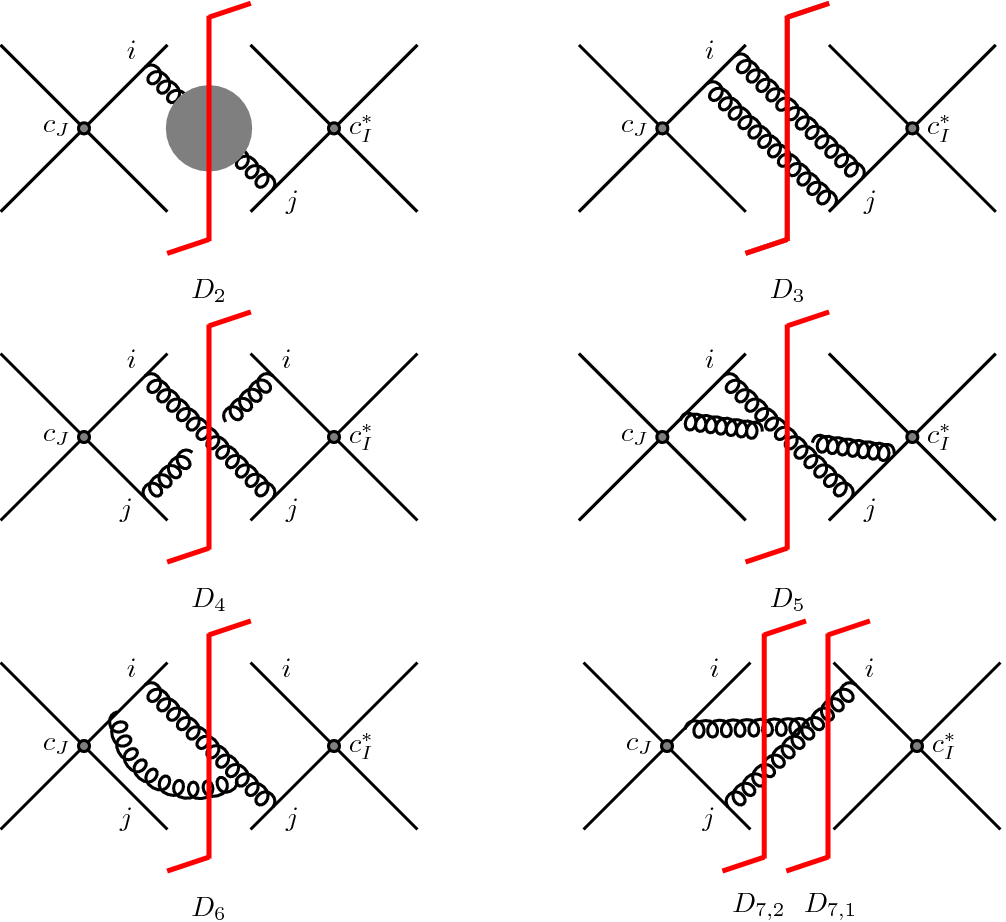
\includegraphics[width=0.7\textwidth]{plots/diagram2-pecjak.png}
%  \end{center}
%  \caption{Two-Wilson-line integrals for the soft function in the massless case.
%  Figure from~\cite{Ferroglia:2012uy}. Our expressions for \ttbar production
%  correspond to diagrams with the gluons attached to both initial
%  (massless) and final (massive) Wilson lines.}
%  \label{fig:pecjak2}
%\end{figure}
%
%The relevant integrals correspond to diagrams of Fig.~\ref{fig:pecjak2}, taken
%from Ref. ~\cite{Ferroglia:2012uy}. 
%%
%The expressions read
%%
%\begin{subequations}
%  \label{eq:2WLIset}
%  \begin{align}
%    %%%
%    I_{3, ij} &= 
%    (n_i \cdot n_j)^2
%    \int \dd^d k\, \dd^d l\; 
%    \frac{\delta_+(k^2) \, \delta_+(l^2)\,
%      \; \delta(q_\perp-|\vec k_\perp+\vec l_\perp |)}
%      {(n \cdot k \, n \cdot l)^\alpha \; 
%      n_i \cdot k \; n_i \cdot
%      (k+l) \; n_j \cdot l \; n_j \cdot (k+l)} \, ,
%    \\[0.7em]
%    %%%
%    I_{4, ij} &= 
%    (n_i \cdot n_j)^2
%    \int \dd^d k\, \dd^d l\; 
%    \frac{\delta_+(k^2) \, \delta_+(l^2) \,
%      \; \delta(q_\perp-|\vec k_\perp+\vec l_\perp |)}
%      {(n \cdot k \, n \cdot l)^\alpha \;
%      n_i \cdot k \; n_i \cdot l \;
%      n_j \cdot k \; n_j \cdot l} \, ,
%    \\[0.7em]
%    %%%
%    I_{5, ij} &=
%    (n_i \cdot n_j)^2
%    \int \dd^d k\, \dd^d l\; 
%    \frac{\delta_+(k^2) \, \delta_+(l^2) \,
%      \; \delta(q_\perp-|\vec k_\perp+\vec l_\perp |)}
%      {(n \cdot k \, n \cdot l)^\alpha  \;
%      n_i \cdot k \; n_i \cdot
%      (k+l) \; n_j \cdot k \; n_j \cdot (k+l)} \, , 
%    \\[0.7em]
%    %%%
%    \label{eq:I6ij}
%    I_{6,ij} &=
%    n_i \cdot n_j
%    \int \dd^d k\, \dd^d l\; 
%    \frac{n_i \cdot (l-k) \;\delta_+(k^2) \, \delta_+(l^2) \, 
%     \delta(q_\perp-|\vec k_\perp+\vec l_\perp |)}
%      {(n \cdot k \, n \cdot l)^\alpha  \;
%      n_i \cdot k \; n_i \cdot (k+l) \; n_j \cdot (k+l) \; (k+l)^2} \, , 
%    \\[0.7em]
%    %%%
%    \label{eq:I72ij}
%    I_{7,2, ij} &=
%    n_i \cdot n_j
%    \int \dd^d k\, \dd^d l\; 
%    \frac{n_j \cdot (k+2l) \; \delta_+(k^2) \, \delta_+(l^2) \,
%      \delta(q_\perp-|\vec k_\perp+\vec l_\perp |)}
%      {(n \cdot k \, n \cdot l)^\alpha  \;
%      n_i \cdot k \; n_j \cdot (k+l) \; n_j \cdot l \; (k+l)^2} \, .
%  \end{align}
%\end{subequations}
%%
%where
%\begin{equation}
%  n_1 = n,     \qquad \qquad
%  n_2 = \nbar, \qquad \qquad
%  n_3 = \tilde v_3,   \qquad \qquad
%  n_4 = \tilde v_4\,.
%  \label{eq:nnlo-external-particles}
%\end{equation}
%%
%We note that the above integrals are invariant under rescaling of external
%momenta. This will be also true for three- and four-Wilson-line integrals.
%Hence, we can work with $v_{3,4}$ or $\tilde v_{3,4}$. We choose the latter as
%it leads to more compact expressions.
% 
%For the time being, we put aside $I_{2, ij}$ and 
%$I_{7,1, ij}$ as they are effectively expressible in terms of 1-loop integrals.
%These cases will be discussed in next section.
%
%In the massless case, all diagonal terms vanish, as they are proportional to
%$n_i^2 = 0$. (This originates from the use of dimensional regularization in
%which scaleless integrals are zero.) In \ttbar production, this is certainly true
%for the incoming particles, hence for $i=1,2$, whereas the other two diagonal
%integrals with $i=3,4$ are in general non-zero.~\footnote{
%There are certainly other symmetries between those integrals, which we can
%study later.
%%
%In particular, there is a chance that, since we adopted the analytic regularization scheme
%of~\cite{Li:2013mia}, the integrals $I_{12}$ and $I_{21}$ are also
%scaleless and vanish as well~(see~\cite{Becher:2010tm}). 
%%
%This was true at NLO but here would need to be checked directly. For the time
%being, we assume that those integrals do not vanish.
%%
%As mentioned in~\cite{Li:2013mia}, vanishing of  $I_{12 (21)}$ integrals in
%certain scheme does not break scheme-independence as those integrals can be
%absorbed into collinear sectors~\cite{Li:2013mia}, hence disappear, in any
%scheme.
%}
%%
%More specifically, the five sets of integrals given in Eqs.~(\ref{eq:2WLIset})
%have the following structure
%%
%\begin{subequations}
%  \begin{align}
%    I_{3, ij},\ I_{5, ij},\ I_{6, ij} &= 
%    \left(
%    \begin{array}{cccc}
%    0      & I_{12} & I_{13} & I_{14} \\
%    I_{21} & 0      & I_{23} & I_{24} \\
%    I_{31} & I_{32} & I_{33} & I_{34} \\
%    I_{41} & I_{42} & I_{43} & I_{44} 
%    \end{array}
%    \right)\,,
%    \\[0.7em]
%    %%%
%    I_{4, ij},\ I_{7,2, ij} &= 
%    \left(
%    \begin{array}{cccc}
%    0      & I_{12} & I_{13} & I_{14} \\
%    I_{21} & 0      & I_{23} & I_{24} \\
%    I_{31} & I_{32} & 0      & I_{34} \\
%    I_{41} & I_{42} & I_{43} & 0 
%    \end{array}
%    \right)\,.
%  \end{align}
%  %\label{eq:}
%\end{subequations}
% 
%Vanishing of $I_{11}$ and $I_{22}$ has been explained above. The reason why there
%are no $I_{33}$ and $I_{44}$ integrals in the second matrix is clear by looking
%at the corresponding diagrams in Fig.~\ref{fig:pecjak2}. 
%
%Setting $i=j$ in $D_4$ or $D_{7,2}$ would turn them into $D_5$ and $D_6$,
%respectively. But the corresponding expressions from Eqs.~(\ref{eq:2WLIset})
%would be wrong since, \eg $D_4$ corresponds to a product of four different
%Wilson lines, expanded to order $g_s$, whereas $D_5$ represents two Wilson
%lines, each expanded to order $g_s^2$. So, the diagonal expressions for
%$I_{4, ij}$ and $I_{7,2, ij}$ simply make no sense and should not be calculated.
%%
%Another way to see this is by noticing that $D_4$ is in fact a convolution of
%two NLO soft functions as none of the momenta attaches to the same
%line twice.
%
%
%
%%-----------------------------------------------------------------------------
%\subsubsection{Three-Wilson-line integrals}
%
%
%From Fig.~\ref{fig:pecjak3} and the Feynman rules of sec.~\ref{sec:FRsoft} we
%deduce the following integrals~\cite{Ferroglia:2012uy} 
%%
%\begin{subequations}
%  \label{eq:3WLIset}
%  \begin{align}
%    %%%
%    I_{8, ijk}^{(a)+(b)} &= 
%    n_i \cdot n_j\; n_i \cdot n_k\; 
%    \int \dd^d k\, \dd^d l\; 
%    \frac{\delta_+(k^2) \, \delta_+(l^2)\,
%      \; \delta(q_\perp-|\vec k_\perp+\vec l_\perp |)}
%      {(n \cdot k \, n \cdot l)^\alpha \; 
%      n_i \cdot k \; n_i \cdot l \; n_j \cdot k \; n_k \cdot l} \, ,
%    \\[0.7em]
%    %%%
%    I_{8, ijk}^{(c)+(d)} &= 
%    n_i \cdot n_j\; n_i \cdot n_k\; 
%    \int \dd^d k\, \dd^d l\; 
%    \frac{\delta_+(k^2) \, \delta_+(l^2)\,
%      \; \delta(q_\perp-|\vec k_\perp+\vec l_\perp |)}
%      {(n \cdot k \, n \cdot l)^\alpha \; 
%      n_i \cdot l \; n_i \cdot (k+l) \; n_j \cdot k \; n_k \cdot l} \, ,
%    \\[0.7em]
%    %%%
%    I_{8, ijk}^{(e)+(f)} &= 
%    n_i \cdot n_j\; n_i \cdot n_k\; 
%    \int \dd^d k\, \dd^d l\; 
%    \frac{\delta_+(k^2) \, \delta_+(l^2)\,
%      \; \delta(q_\perp-|\vec k_\perp+\vec l_\perp |)}
%      {(n \cdot k \, n \cdot l)^\alpha \; 
%      n_i \cdot k \; n_i \cdot (k+l) \; n_j \cdot k \; n_k \cdot l} \,,
%  \end{align}
%\end{subequations}
%%
%and the external particles are defined as in
%Eq.~(\ref{eq:nnlo-external-particles}).
%%
%Each of the above integrals is proportional to a different colour factor.
%
%\begin{figure}[t]
%  \begin{center}
%    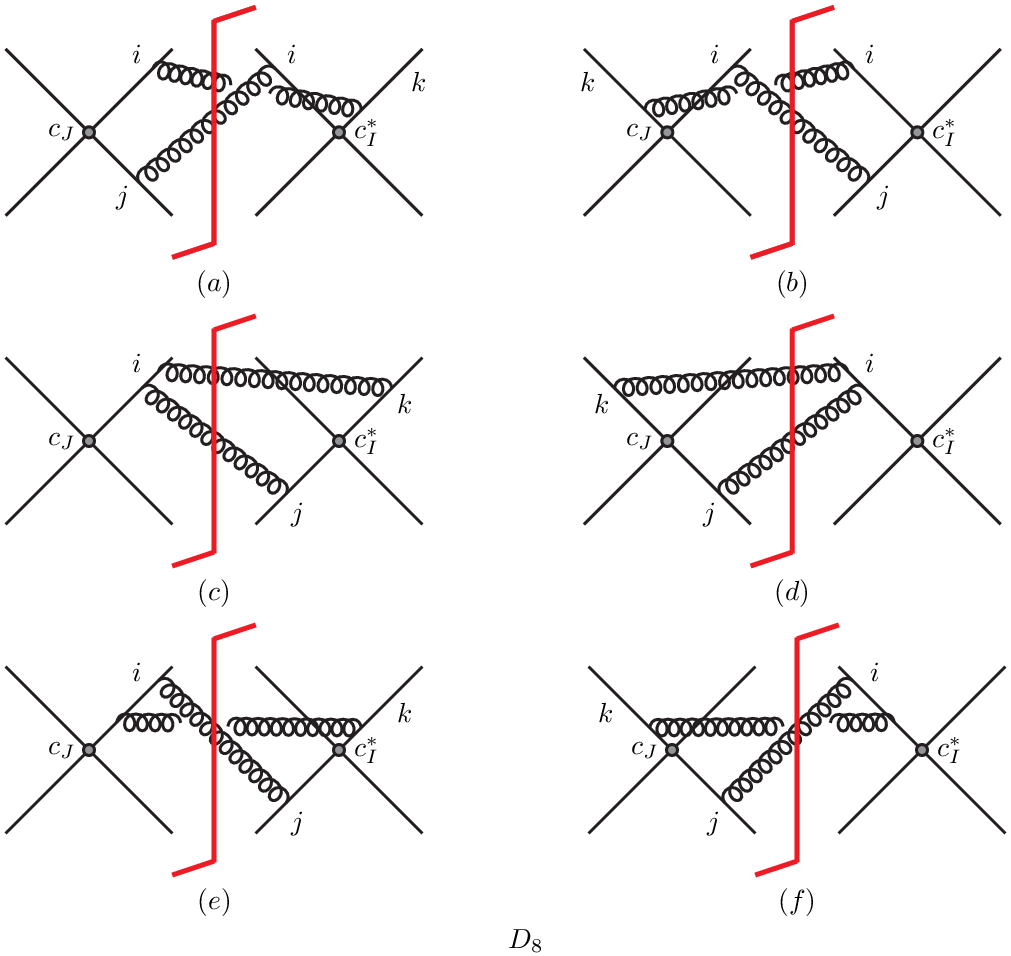
\includegraphics[width=0.7\textwidth]{plots/diagram3-pecjak.png}
%  \end{center}
%  \caption{
%    Three-Wilson-line integrals, the abelian case.
%  }
%  \label{fig:pecjak3}
%\end{figure}
%%
%\begin{figure}[t]
%  \begin{center}
%    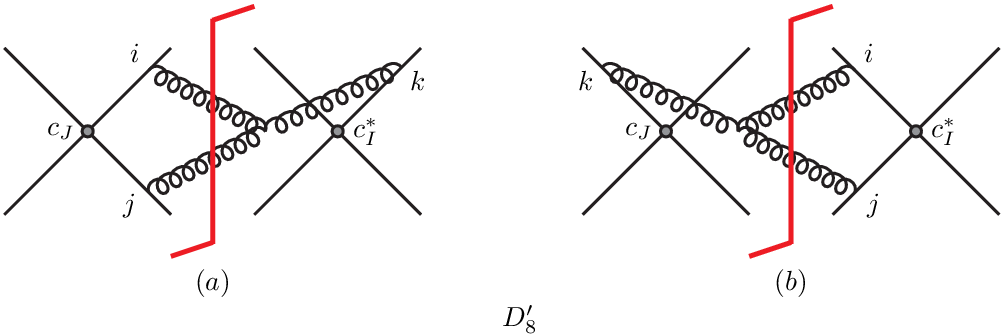
\includegraphics[width=0.7\textwidth]{plots/diagram5-pecjak.png}
%  \end{center}
%  \caption{
%    Three-Wilson-line integrals, the non-abelian case.
%  }
%  \label{fig:pecjak5}
%\end{figure}
%
%Diagrams $(a)$ and $(b)$ are again convolutions of NLO soft functions, hence we
%set all the diagonal terms: $I_{iik}, I_{iji}, I_{ijj}$ to zero. 
%%
%As for $(c), (d), (e)$ and $(f)$, we may have $I_{iik}, I_{iji}$ but not
%$I_{ijj}$, as the latter would involve only two Wilson lines. Of the first two,
%the integrals do not vanish only if $i=3,4$. In summary, the three-Wilson-lines
%integrals given in Eqs.~(\ref{eq:3WLIset}) and represented by diagrams in
%Fig.~\ref{fig:pecjak3} are non-vanishing except for
%%
%\begin{equation}
%  \begin{array}{ccc}
%  I^{(a,b)}_{8,ijk} = 0     & \quad \text{if} \quad & 
%                               i=j\ \lor\ i=k\ \lor\ j=k\,,
%  \\[0.5em]
%  I^{(c,d,e,f)}_{8,ijk} = 0 & \quad \text{if} \quad & j=k\,,
%  \\[0.5em]
%  I^{(c,d,e,f)}_{8,ijk} = 0 & \quad \text{if} \quad & 
%                              (i=j\ \lor\ i=k)\ \land\ (i=1\ \lor\ i=2)\,.
%  \end{array}
%  %\label{eq:}
%\end{equation}
%
%There is also a group of non-abelian integrals like those shown in
%Fig.~\ref{fig:pecjak5}. The sum of those two diagrams vanishes due to colour
%structure as, following the Feynman rules discussed earlier, we have
%%
%\begin{subequations}
%  \begin{align}
%   D'^{(a)}_8 &\propto i f^{abc}\, T_i^a\, T_j^b\, T_k^c\, I'_8\,, \\
%   D'^{(b)}_8 &\propto -i f^{abc}\, T_i^a\, T_j^b\, T_k^c\, I'_8\,.
%  \end{align}
%  %\label{eq:}
%\end{subequations}
%%
%The relative minus sign comes from the fact that the gluon propagator carrying
%momentum $k+l$ appears on opposite sides of the cut in the two diagrams
%(see sec.~3.2 in ~\cite{Ferroglia:2012uy} for further discussion).
%%
%The same is true for one-particle cut diagrams analogous to those of
%Fig.~\ref{fig:pecjak5}.
%
%
%
%%-----------------------------------------------------------------------------
%\subsubsection{Four-Wilson-line integrals}
% 
%\begin{figure}[t]
%  \begin{center}
%    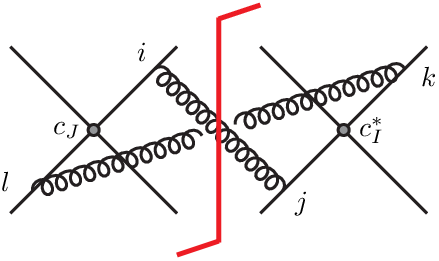
\includegraphics[width=0.35\textwidth]{plots/diagram6-pecjak.png}
%  \end{center}
%  \caption{
%    Four-Wilson-line integrals.
%  }
%  \label{fig:pecjak6}
%\end{figure}
%
%Finally, we have the integrals corresponding to Fig.~\ref{fig:pecjak6}, with 
%four different gluon attachments~\cite{Ferroglia:2012uy}
%%
%\begin{align}
%  %%%
%  \label{eq:4WLIset}
%  I_{9, ijkl} &= 
%  n_i \cdot n_j\; n_k \cdot n_l\; 
%  \int \dd^d k\, \dd^d l\; 
%  \frac{\delta_+(k^2) \, \delta_+(l^2)\,
%    \; \delta(q_\perp-|\vec k_\perp+\vec l_\perp |)}
%    {(n \cdot k \, n \cdot l)^\alpha \; 
%    n_i \cdot k \; n_j \cdot k \; n_k \cdot l \; n_l \cdot l} \,.
%\end{align}
%
%Some of the indices have a chance to be equal and render the integral non-zero
%provided that the gluons are attached to four distinct Wilson lines and, as
%usual, only the squares of massive vectors, hence $n_i^2$ with $i=3,4$, survive.
%On the other hand, if the two indices on the same side of the cut become equal,
%that corresponds to three-Wilson-lines diagram and should be rejected.
%We can summarize the above by
%%
%\begin{equation}
%  \begin{array}{ccc}
%  I_{9, ijkl} = 0  &\quad \text{if} \quad & (i=j\ \land\ i = 1,2)\ \lor\
%                                            (k=l\ \land\ k = 1,2)\,,
%  \\[0.5em]
%  I_{9, ijkl} = 0  &\quad \text{if} \quad & i=l\ \lor\ k=j\,.
%  \end{array}
%  %\label{eq:}
%\end{equation}

%------------------------------------






%-----------------------------------------------------------------------------
\bibliographystyle{unsrt}
\bibliography{precision-qcd2}

\end{document}
